\documentclass[
  a4paper, 
  12pt,
  ja=standard,
  xelatex,
  left=30truemm,
  right=30truemm,
  titlepage 
]{bxjsarticle}

\title{Kashiwara crystal と  Robinson-Schensted-Knuth \\ 対応の関係 \\[50pt]}
\author{
  アドバイザー:岡田聡一教授\\[20pt]
  322301150 \quad 菊地雄大
}
\date{}

\usepackage{amsmath, amssymb, amsthm, mathrsfs}
\usepackage{ytableau}
\usepackage{xeCJK}
\usepackage{fontspec}
\usepackage{tikz}
\usetikzlibrary{arrows.meta}
\usepackage{tikz-cd}
\usepackage[utf8]{inputenc}
\newcommand{\amp}{&}
\usepackage{latexsym}
\def\proofname{\textbf{証明}}
\ytableausetup{centertableaux,mathmode}

\theoremstyle{definition}
\newtheorem{df}{定義}[section]
\newtheorem{thm}{定理}[section]
\newtheorem{prop}[thm]{命題}
\newtheorem{cor}[thm]{系}
\newtheorem{lem}[thm]{補題}
\newtheorem*{ex}{例}
\newtheorem*{re}{注意}

\begin{document}

\maketitle
\thispagestyle{empty}

\pagenumbering{arabic}
\setcounter{page}{1}

\tableofcontents
\clearpage

\section{イントロダクション}
本論文は, 参考文献 \cite{b2} を基に, 
Kashiwara crystal(以下「crystal」と略す)および Robinson-Schensted-Knuth 対応(以下「RSK対応」と略す)の概要と 
それらの関係性についてのサーベイを行うものである.
分割とは正整数を他の正整数の和として表現する方法である.
例えば, $3$ の分割を考えると, $3$ という数を $3, 2 + 1, 1 + 1 + 1$ の3種類で, 他の正整数の和として表せる.
これをそれぞれ $(3), (2, 1), (1^3)$ と表現するのが分割という概念である.
この分割を視覚的に表現する方法として, Ferrers diagram と呼ばれる概念がある.
$\lambda = (\lambda_1, \lambda_2, \cdots, \lambda_l)$ をある分割としたときに, 
$i$ 行に $\lambda_i$ 個の箱を左寄せで書いたものを 形 $\lambda$ のFerrers diagramという.
その箱の中に正整数を1つづつ書いたものが tableau である.
形 $(2, 1)$ の Ferrers diagram と tableau として
\[
\ytableaushort{~~,~} \qquad
\ytableaushort{12,3}
\]
がある.
Robinson Schensted Knuth 対応とは
word(文字列) を tableau の組に写す写像である. 
例えば, 
$$13221 
\rightarrow
\left( 
  \ytableaushort{112,1,3}
 \mathrel{,} 
  \ytableaushort{124,3,5}
\right)
$$
のようである.
第1成分を P-tableau, 第2成分を Q-tableau という.

Kashiwara crystal は, 柏原正樹によって導入されたもので, 
表現論を視覚的かつ組合せ論的に解析するためのツールである.
crystal は, ある集合とその上の構造で定義されたもので,
\begin{enumerate}
  \item 各元は weight を持つ.
  \item 作用素 $e_i$ と $f_i$ を持ち, これらは crystal の元の間での遷移を定義する.
  \item 各元 $b$ について, $\varphi_i(b)$ と $\varepsilon_i(b)$ という整数値が定義される.
  通常, $\varphi_i(b)$ は $f_i$ を適用して遷移可能な回数,
  $\varepsilon_i(b)$ は $e_i$ を適用して遷移可能な回数 を表す.
\end{enumerate}
を満たすものである. これを視覚的に表現する方法として, crystal graph がある.
$A_r$ 型のcrystal $\mathbb{B}$ は, crystal graph として,
\[
  \ytableaushort{1}
  \xrightarrow{1}
  \ytableaushort{2}
  \xrightarrow{2}
  \cdots
  \xrightarrow{r}
  \begin{ytableau}
    \scriptstyle{r + 1}
  \end{ytableau}
\]
を持つ. 
本論文では, この $k$ 回のテンソル積によって構成される crystal 
$$
\mathbb{B}^{\otimes k} = \{ x_1 \otimes \cdots \otimes x_k \mid x_1, \cdots, x_k \in \{ 1, \cdots, r + 1 \} \}
$$
に着目する.
この crystal $\mathbb{B}^{\otimes k}$ を連結な crystal の直和に分解することを考える.  
同じ形を持つ semistandard tableau 全体が1つの連結な crystal を構成し, その直和として $\mathbb{B}^{\otimes k}$ を表すことができる.

この $\mathbb{B}^{\otimes k}$ の元 $x = x_1 \otimes \cdots \otimes x_k$ に対して, P-tableau $P(x)$ を考える.  
このとき, 以下の定理(本文の定理 \ref{crystal-and-p-tableau})が成り立つ.

\begin{thm}[{\cite[定理8.6]{b2}}]
  crystal $\mathbb{B}^{\otimes k}$ を tableau の crystal の直和に分解する.
  このとき, $x$ は分解された crystal の中で $P(x)$ に対応している.  
  したがって, $P(x)$ の形が $\lambda$ であるとき, $x$ は 形 $\lambda$ の連結な tableau の crystal の元に対応している.
\end{thm}

一方, $\mathbb{B}^{\otimes k}$ を連結な tableau の crystal に分解すると, 直和の各成分に重複が存在する.  
そのため, $x, y \in \mathbb{B}^{\otimes k}$ の P-tableau の形が一致していたとしても, 必ずしも同じ連結な tableau の crystal に対応しているとは限らない.  
しかし, Q-tableau を考えることで, 以下の定理(本文の定理 \ref{crystal-and-q-tableau})が導かれる.

\begin{thm}[{\cite[定理8.7]{b2}}]
  $x, y \in \mathbb{B}^{\otimes k}$ の Q-tableau が一致するとき, 
  $x, y$ は $\mathbb{B}^{\otimes k}$ の同じ連結成分に属している.
\end{thm}

このように, P-tableau と Q-tableau は, この crystal 構造において重要な役割を果たしている.

本論文では, Robinson-Schensted-Knuth 対応, Kashiwara crystal, 上記で述べたこの2つの関係性について,
順を追って議論していく.
まず, RSK対応に関して, 分割および tableau の基本的な定義を行い, 
これらを用いた insert 操作および RSK 対応のアルゴリズムを紹介する.
さらに, RSK対応における重要な概念である Knuth 同値および P-同値 について論じる.
Knuth 同値は, 2つの P-tableau が一致するときの word 間の関係性を述べたものである.
次に, 鏡映, weight, ルート系といった基礎概念を定義した後, 
Kashiwara crystal について説明する.
続いて, crystal の準同型写像およびテンソル積の構造について詳述する. 
さらに,  $\mathbb{B}^{\otimes k}$ の計算手法として signature rule を紹介する.
最後に, crystal と RSK 対応の関係性を考察する. 
その際, tableau に対応する crystal の構造とその最高 weight 元との関係を明らかにする.
上記で述べた crystal と RSK 対応の関係性を説明するために
plactically 同値 を定義し, 証明するときの鍵となる Knuth 同値との関連性を説明する.

\begin{center} \textbf{[使用記号について]} \end{center}

$\mathbb{R}$ : 実数全体, $\mathbb{Z}$ : 整数全体を表す.
$k$ を正整数とし, $[k] = \{ 1, 2, \cdots, k \}$ とする.

\section{Robinson-Schensted-Knuth 対応}
Robinson-Schensted-Knuth (RSK) 対応は, 組合せ論や表現論において重要なアルゴリズムである.
1938年に Gilbert de Beauregard Robinson が最初に提案し, 
その後Craige Eugene Schensted や Donald Ervin Knuth によって発展・一般化された.
この功績により, このアルゴリズムは Robinson-Schensted-Knuth 対応と名付けられている.
RSK 対応は, 行列や一般化置換などの構造から, tableau の組への変換を行うアルゴリズムである.
変換の対象となるものは様々であるが, ここでは word を対象とし, 説明する.

以下では, RSK 対応を定義するのに必要な概念である分割と tableau の定義を最初に説明する.
その後, RSK 対応のアルゴリズムを説明し, その性質として Knuth 同値とP-同値の関係性について述べる.

\subsection{分割と tableau の定義}
まず分割を定義する.
\begin{df}
  $\lambda = (\lambda_1, \lambda_2, \cdots, \lambda_l)$ が $k$ の分割であるとは,
  \begin{enumerate}
    \item $\lambda_i$ は正整数, $\sum_{i=1}^l \lambda_i=k$
    \item $\lambda_1\geq \lambda_2  \geq \cdots \geq  \lambda_l$ 
  \end{enumerate}
  を満たすときをいう. 
  このとき,  $\lambda \vdash k$ で表す.
\end{df}

分割を表記する際, 同じ数が繰り返される部分については累乗記法を用いて表すことがある.
例えば, $(3, 1, 1)$ を $(3, 1^2)$ で表す.

\begin{ex}
  $5$ の分割は, $(5), (4, 1), (3, 2), (3, 1^2), (2^2, 1), (2, 1^4), (1^5)$ の7つである.
\end{ex}

次に, Ferrers diagram と tableau を定義する.
分割 $\lambda$ を図式的に表現する方法として, 形 $\lambda$ の Ferrers diagram がある.
その diagram の各箱の中に数字を入れたものが tableau である.

Ferrers diagram は 数学者 Norman Macleod Ferrers に由来し, 
Young tableau は 1900 年に 数学者 Alfred Young によって名付けられたものである.

\begin{df} $\lambda = (\lambda_1, \lambda_2, \cdots, \lambda_l) \vdash k$ とする.
  \begin{enumerate} 
    \item 形 $\lambda$ の Ferrers diagram とは, $i$ 行に $\lambda_i$ 個の箱を左寄せに書いた並びである. 
    $i$ 行 $j$ 列の箱は座標 $(i, j)$ を持つ.
    \item 形 $\lambda$ の Young tableau とは Ferrers diagram の各箱内に $[k]$ 内の元を1回ずつ書いた並びである. 
    この並びが各行, 各列に関して単調増加であるとき, standard tableau であるという.
    \item 形 $\lambda$ の generalized Young tableau とは Ferrers diagram の各箱内に正整数を繰り返しを許して書いた並びである. 
    この並びが各行に関して広義単調増加, 各列に関して狭義単調増加であるとき, semistandard tableau であるという.
  \end{enumerate} 
\end{df}

この定義から, 形 $\lambda$ の standard tableau の成分は $k$ 以下の正整数であり,
その個数は有限個である.
一方, 形 $\lambda$ の semistandard tableau の成分は $k$ より大きい数も入り,
無限に存在する.
そこで $n$ を正整数とし, 成分の値が $n$ 以下の semistandard tableau を今後は考えていく.

また, Young tableau は generalized Young tableau の特殊な場合であることに注意する.

\begin{ex}
  $\lambda=(3, 2, 1) \vdash 6$ のFerrers diagramは
  \[
    \ytableaushort{~~~,~~,~}
  \]
  である. 
  standard tableau は, 例えば以下がある.
  \[
    \ytableaushort{123,45,6} \quad
    \ytableaushort{134,26,5} \quad
    \ytableaushort{125,36,4}
  \]
  この standard tableau は semistandard tableau でもある.
  これ以外に semistandard tableau は, 例えば以下がある.
  \[
    \ytableaushort{111,22,3} \quad
    \ytableaushort{122,23,3} \quad
    \ytableaushort{357,57,7}
  \]
  \\[10pt]
\end{ex}

次の概念は, 後にある節の Knuth 同値と P-同値の関係性について証明する際や
tableau の crystal を考える際に役に立つ.

\begin{df}
  $T$ を Young tableau または generalized Young tableau とする.
  $T$ の行を1行目から順に $T_1, T_2, \cdots, T_l$ とする.

  $T$ の row word $\pi_T$ を
  $$ \pi_T = T_l T_{l-1} \cdots T_1 $$
  と定める.
\end{df}

\begin{ex}
  $T = \ytableaushort{123, 45, 6}$ とする. 
  このとき,
  $$ \pi_T = 645123 $$
  である.
\end{ex}

\subsection{insertion と Robinson-Schensted-Knuth 対応}
Robinson-Schensted-Knuth 対応 を定義するのに必要な insertion について説明する.
insertion は, tableau に数を追加することで, 新たな tableau を生成する方法である.

\begin{df}
  $T$ を semistandard tableau, $i$ を任意の正整数とする.
  $T$ に $i$ を insert するとは以下の手順を行うことである.
  \begin{enumerate}
    \item $T$ の1行目を $R$ とする.
    \item $R$ 内の成分で $i$ より大きい成分があるとき, 次の (2a) から (2c) の操作を繰り返す.
    \begin{enumerate}
        \item[(2a)] $R$ 内の成分を左から右へ順に見ていき, $i$ より大きい最初の成分を $j$ とする.
        \item[(2b)] $j$ を $i$ と入れ替える. (すなわち, $j$ を取り出して $i$ をその位置に置く).
        \item[(2c)] $i$ を更新して $i := j$ とし, $R$ を次の行とする.
    \end{enumerate}
    \item $R$ 内に $i$ より大きい成分が存在しない ($R$ 内のすべての成分が $i$ 以下) のとき, その行の最後の列に $i$ を追加し, 操作を終了する.
  \end{enumerate}
  この操作により得られた generalized Young tableau を $T \leftarrow i$ で表す.
\end{df}

\begin{ex}
  $T = \ytableaushort{23346, 357}$ に $3$ を insert すると, 次の操作が行われる.
  \begin{align*}
    & T = \ytableaushort{23346, 357} \quad (\text{最初の tableau}) \\
    & \rightarrow 
    \ytableaushort{23336, 357} \quad (\text{1行目に $3$ を挿入し, $4$ を押し出す. }) \\
    & \rightarrow
    \ytableaushort{23336, 347} \quad (\text{2行目に $4$ を挿入し, $5$ を押し出す. }) \\
    & \rightarrow
    \ytableaushort{23336, 347, 5} \quad (\text{3行目に $5$ を追加し, 操作を終了する. })
  \end{align*}
\end{ex}

次に, Robinson-Schensted-Knuth 対応を定義する.

\begin{df}
  $n$ と $k$ を正の整数とする.
  Robinson-Schensted-Knuth 対応とは, アルファベット $[n]$ 上の長さ $k$ の word $w = i_1 i_2 \cdots i_k$ に対して,
  以下で定まる同じ形の generalized Young tableau $P$ と Young tableau $Q$ の組 $(P,Q)$ を対応させる写像である.
  \begin{itemize}
    \item $P$ は $ \varnothing \leftarrow i_1 \leftarrow i_2 \leftarrow \cdots \leftarrow i_k $
    \item $Q$ は, $P$ に $i_s$ を insert した際に新しく追加された箱と同じ成分を持つ箱に $s$ を書き込む.
    (ただし, $1 \leq s \leq k$ とする.)
  \end{itemize}
  このとき, $P$ を P-tableauといい, $P(w)$ で表す.
  同様に, $Q$ を Q-tableauといい, $Q(w)$ で表す.
\end{df}

以下, Robinson-Schensted-Knuth 対応を RSK 対応と略す.

\begin{ex}
  $w = 3 2 2 5 1$とする.
  このとき,
  \[
  P: \varnothing \overset{3}{\rightarrow} 
  \ytableaushort{3} \overset{2}{\rightarrow}
  \ytableaushort{2, 3} \overset{2}{\rightarrow}
  \ytableaushort{22, 3} \overset{5}{\rightarrow}
  \ytableaushort{225, 3} \overset{1}{\rightarrow}
  \ytableaushort{125, 2, 3}
  \]
  \[
  Q: \varnothing \rightarrow
  \ytableaushort{1} \rightarrow
  \ytableaushort{1, 2} \rightarrow
  \ytableaushort{12, 3} \rightarrow
  \ytableaushort{124, 3} \rightarrow
  \ytableaushort{124, 3, 5}
  \]
  となる.
\end{ex}

次の定理は重要である.

\begin{thm} [{\cite[定理4.8.2]{b1}}] 
  \begin{enumerate}
    \item[]
    \item P-tableau は semistandard tableau, Q-tableau は standard tableau である.
    \item RSK 対応は, アルファベット $[n]$ 上の長さ $k$ の word 全体の集合から, $k$ の分割の形で
    $[n]$ 上の元を成分にもつ semistandard tableau $P$ と standard tableau $Q$ の組 $(P,Q)$ 全体の集合への全単射である.
    \item $P(\pi_T) = T$
  \end{enumerate}
\end{thm}

\begin{proof}
  \begin{enumerate}
    \item[] 
    \item Q-tableau が standard tableau であることは定義から明らかである. P-tableau が semistandard であることは, 
    semistandard tableau $T$ と任意の $i$ に対し, $T \leftarrow i$ が semistandard であることを示せば十分である.
    $T \leftarrow i$ が行に関して広義単調増加であることは明らかである. 列に関して狭義単調増加であることは, ある列で $m + 1$ が
    押し出され, $m$ が insert されたとき, その上にある成分が $m$ ではないことを確認すれば良い. ある列で $m + 1$ が
    押し出され, $m$ が insert されたと仮定する. この $m$ が insert された座標を $(i, j)$ とすると, 
    それが insert する前に $i - 1$ 行では, $j -1$ 列より前で $m$ があり, それが押し出されたことで
    $i$ 行目で $m$ が insert されたことになる. したがって, $(i, j-1)$ 成分は, $m$ より大きく, $m + 1$ 以下であるから, $m + 1$
    となる. よって, $(i, j)$ で $m$ が押し出されたことに矛盾する. 
    \item 逆写像が存在することを示せば良い. 
    $$(P, Q) = (P_k, Q_k) \rightarrow (P_{k -1}, Q_{k -1}) \rightarrow \cdots \rightarrow (\varnothing, \varnothing)$$
    を以下のようにして, $m$ 番目から $m -  1$ 番目を構成する. \\
    (1) $(i, j)$ を $Q_m$ 内で $m$ の成分がある座標とし, $Q_m$ から $m$ を取り除いた tableauを $Q_{m - 1}$ とする.
    $x$ を $P_{m}$ の $(i, j)$ 成分の値, $R$ を $P_{m}$ の $i - 1$ 行とする. \\
    (2) $R$ が $P_{m}$の 0行でないとき, \\
    \quad (2a) $y$ を $x$ より小さい元 $R$ の元の内で一番右側にある元とし, $R$ 上で $y$ を $x$ \\
    \quad に置き換える. \\
    \quad (2b) $x$ の値を更新して $x$ の値を $y$ とし, $R$ を 1行上の行とする. \\
    (3) $x$ を $P_{m}$の $1$ 行目から取り除き, これを $Q_{m -1}$ とする. この $x$ を $i_m$ とする. \\
    この操作でできた $w = i_1 i_2 \cdots i_k$ を $(P, Q)$ からの値とすると, この対応が逆写像になる.
    \item 明らかである.
  \end{enumerate}
\end{proof}

\subsection{Knuth 同値と P-同値}
この節では, P-tableau に着目する.
2つの word の P-tableau が一致するときの
word の関係性を述べたのが Knuth 関係である.

\begin{df} $w_1, w_2$ を word とする.
  \begin{enumerate}
    \item $w_1$ が $w_2$と Knuth 関係であるとは,  
    $$ w_1 = ....bca... \ , \quad w_2 = ...bac... \quad (a < b \leq c)$$
    または
    $$ w_1 = ....acb... \ , \quad w_2 = ...cab... \quad (a \leq b < c)$$
    であるとき (または $w_1, w_2$ が逆のとき) をいう. \\
    (ただし, $...$ 部分は $w_1$ と $w_2$ が一致していることを意味する. )
    \item $w_1$ が 有限回の Knuth 関係による置き換えを適用することで $w_2$ ができるとき,
    $w_1$ と $w_2$ は Knuth 同値であるという. このとき, $w_1 \equiv_{K} w_2$ で表す.
  \end{enumerate}
\end{df}

\begin{ex}
  $w = 2 1 3 2$とする.
  \[
    2 1 3 2 \equiv_{K} 2 3 1 2 \equiv_{K} 3 2 1 2 \equiv_{K} 3 1 2 2
  \]
  である.
\end{ex}

\begin{df}
  $w_1, w_2$ を word とする.
  $P(w_1) = P(w_2) $であるとき, $w_1, w_2$は P-同値であるといい, $w_1 \equiv_{P} w_2 $ で表す.
\end{df}

\begin{ex}
  $w_1 = 2 1 3 2, w_2 = 3 1 2 2 $とする.
  $$ P(w_1) = \ytableaushort{12,23} = P(w_2) $$
  であるから, $w_1 \equiv_{P} w_2 $ である.
\end{ex}

\begin{thm} [{\cite[定理3.4.3]{b1}}] \label{k-p-equiv}
  $w_1, w_2$ を word とする.
  $w_1 \equiv_{K} w_2$ であることと $w_1 \equiv_{P} w_2 $ であることは必要十分条件である.
\end{thm}

\begin{proof}
  $ w_1 = ....bca... \ , \quad w_2 = ...bac...(a < b \leq c) $ とする.
  $T$ を $b$ の手前までの元を insert してできた tableau とする.
  このとき,
  $$T \leftarrow b \leftarrow c \leftarrow a = T \leftarrow b \leftarrow a \leftarrow c$$
  を示せば良い.
  $T$ の行の数に関する帰納法で示す.
  $T = \emptyset$ のとき, 上記の insert でできる tableau はともに
  $$\ytableaushort{ac,b}$$
  である.

  次に, $T$ を 1行以上からなる tableau する.
  $T \leftarrow b$ を考え,
  $b$ が $T$ の1行目の $m$ 列にある $b'$ で入れ替わるとする.
  $T \leftarrow b$ に $a$ を insert することを考えると,
  $a < b$ であるから, $a$ は 1行目の $m$ 以下の列に入る.
  このとき, 押し出された元を $a'$ とすると, $a' < b'$ である.
  $T \leftarrow b \leftarrow a$ に $c$ をinsert すると,
  $c \geq b$ であるから, 1行目の $m + 1$ 以上の列に入る.
  このとき, 押し出された元を $c'$ とすると, $c' \geq b'$ である.
  $T \leftarrow b \leftarrow c \leftarrow a$ についても考えると,
  同様のことが起きる.
  よって, $T \leftarrow b \leftarrow c \leftarrow a$ と $T \leftarrow b \leftarrow a \leftarrow c$
  の1行目は一致することが分かる.
  $T'$ を $T$ の1行目を取り除いてできる tableau とすると,
  $$T' \leftarrow b' \leftarrow c' \leftarrow a' = T' \leftarrow b' \leftarrow a' \leftarrow c'$$
  を示せば良いことが分かるが, $T'$ の行が $T$ の行より1つ小さいことと帰納法から従う.

  また, $ w_1 = ....acb... \ , \quad w_2 = ...cab... (a \leq b < c)$ のときについても同様である.
  以上から, $w_1 \equiv_{K} w_2$ ならば $w_1 \equiv_{P} w_2$ が成り立つことが言えた.

  次に, この逆を示す. 任意の word に対して,
  $$w \equiv_{K} \pi_{P(w)}$$
  を示せば十分である. これを利用すると,
  $w_1 \equiv_{P} w_2 $ であるならば,
  $$w_1 \equiv_{K} \pi_{P(w_1)} = \pi_{P(w_2)} \equiv_{K}  w_2$$
  と示せるからである.

  $w$ の元の数に関する帰納法で示す.
  $w$ の最後の元を $x$, $w$ から最後の元を取り除いた word を $w'$ とする.
  即ち, $w = w'x$ である.
  $w'$ の元の数 は $w$ の元の数より1つ小さいから, 帰納法の仮定により,
  $w' \equiv_{K} \pi_{P(w')}$ である.
  $P(w')$ の行を $R_1, \cdots, R_l$, $R_1 = p_1 \cdots p_m$ とする.
  $P(w')$ に $x$ を insert したとき, 1行目の $j$ 列に入るとする.
  このとき,
  \begin{align*}
    \pi_{P(w)} 
    &= \pi_{{P(w')}} x \\
    &= R_l \cdots R_2 p_1 \cdots p_m x \\
    &\equiv_{K} R_l \cdots R_2 p_1 \cdots p_{m - 1} x p_m \\
    &\equiv_{K} \cdots \\
    &\equiv_{K} R_l \cdots R_2 p_1 \cdots p_j x p_{j + 1} \cdots p_m \\
    &\equiv_{K} R_l \cdots R_2 p_1 \cdots p_j p_{j - 1} x p_{j + 1} \cdots p_m \\
    &\equiv_{K} R_l \cdots R_2 p_j p_1 \cdots p_{j - 1} x p_{j + 1} \cdots p_m
  \end{align*}
  となる.
  末尾の $p_1 \cdots p_{j - 1} x p_{j + 1} \cdots p_m$ は
  $P(w') \leftarrow x$ の1行目に一致する.
  先頭の $R_l \cdots R_2 p_j$ の部分は, $P(w') \leftarrow x$ の1行目で押し出された $p_j$ が
  2行目に insert される操作に対応しており, 1行目の時と同様の方法を考えることができる.
  これを2行目以降続けていくことで最終的に, $P(w)$ の row word が得られる.
\end{proof}

\section{Kashiwara crystal}
Kashiwara crystal はリー群の表現を反映する組合せ的構造である.
1990年頃に柏原正樹によって, 量子群の加群が crystal 基底 という特別な基底を持つことが示された.
また, RSK 対応などの tableau の組合せ論における研究も crystal の枠組みで再解釈することが可能である.
特に, $A$ 型の crystal は semistandard tableau と密接に結びついており, 
crystal 上の作用素が tableau に特定の操作を施す形で定義される.
このように, Kashiwara crystal は量子群の表現論と組合せ論を結びつける重要な橋渡しとなっている.

この節では, Kashiwara crystal の定義に必要な鏡映, weight lattice, ルート系を最初に紹介する.
その後, crystal を定義し, tableau の crystal を考える際に必要な概念である crystal 準同型とテンソル積を定義する.
例では, semistandard tableau と密接に結びついている $A$ 型の crystal を中心に紹介する.

以下, $V$ をユークリッド空間とする. すなわち, 内積 $\langle \cdot, \cdot \rangle$ を備えた実ベクトル空間とする. 
例で使用するユークリッド空間は, すべて標準的な内積により定義されるものとする. 
また, $e_i \in \mathbb{R}^r$ は第 $i$ 成分が $1$ で, それ以外の成分が $0$ である標準基底ベクトルを表す.

\subsection{鏡映, weight lattice, ルート系}
Kashiwara crystal の定義に必要な概念である鏡映, weight lattice, ルート系
について説明する.

鏡映とは, ベクトルをある超平面に対して対称に反転させる操作のことである.

\begin{df}
  $0 \neq  \alpha \in V $ の鏡映 $r_\alpha: V \to V $ を
  \[
  r_\alpha (x) = x - \langle x , \alpha^{ \vee } \rangle \quad \left(\text{ただし, } \alpha^{ \vee } = \frac{2 \alpha}{\langle \alpha, \alpha \rangle} \right)
  \]
  とする.
\end{df}

\begin{ex}
  $V = \mathbb{R}^3$ とし $\alpha = (1, 0, -1)$ を考える.

  このとき, $\alpha^{\vee}$ は次のように計算される.
  \[
  \alpha^{\vee} = \frac{2 \alpha}{\langle \alpha, \alpha \rangle} = \frac{2 (1, 0, -1)}{1^2 + 0^2 + (-1)^2} = (1, 0, -1).
  \]

  次に内積 $\langle x, \alpha^{\vee} \rangle$ を計算すると,
  \[
  \langle x, \alpha^{\vee} \rangle = \langle (x_1, x_2, x_3), (1, 0, -1) \rangle = x_1 - x_3.
  \]

  よって, 任意の点 $x = (x_1, x_2, x_3) \in \mathbb{R}^3$ に対する鏡映 $r_\alpha(x)$ は次のように表される.
  \[
  \begin{aligned}
    r_\alpha(x) 
    &= x - \langle x, \alpha^{\vee} \rangle \alpha \\
    &= (x_1, x_2, x_3) - (x_1 - x_3)(1, 0, -1) \\
    &= \left( x_1 - (x_1 - x_3), x_2, x_3 + (x_1 - x_3) \right) \\
    &= \left( x_3, x_2, x_1 \right).
  \end{aligned}
  \]

  例えば,
  $r_\alpha(e_1) = e_3, r_\alpha(e_2) = e_2, r_\alpha(e_3) = e_1$
  である.
\end{ex}

一般に 鏡映 $r_\alpha$ に対し,
$$r_\alpha(\alpha) = \alpha - \langle \alpha, \alpha^{\vee} \rangle \alpha = - \alpha$$
となる. また, $x$ が $\alpha$ に直交するとき,
$$r_\alpha(x) = x - \langle x, \alpha^{\vee} \rangle \alpha = x$$
となる. このような $\alpha$ と直交する空間のことを $\alpha$ に垂直な超平面という.
そのため, 鏡映とは ベクトルをある超平面に対して対称に反転させる操作と言えるのである.

次に, ルート系を定義する.
ルート系は, 鏡映による対称性を持つベクトルの集合である.

\begin{df} 
  $V$ 上のルート系 $\Phi$ を以下を満たす有限集合とする.
  \begin{enumerate}
    \item $ 0 \notin \Phi , \Phi \neq \emptyset $
    \item $ r_\alpha (\Phi) = \Phi \quad ( \alpha \in \Phi )$
    \item $ \langle \alpha, \beta^{ \vee } \rangle \in \mathbb{Z} \quad ( \alpha, \beta \in \Phi )$
    \item $ \beta \in \Phi $ が $ \alpha \in \Phi $ のスカラー倍であるならば, $ \beta = \pm \alpha $ である.
  \end{enumerate}
  このとき, $ \Phi $の元をルートという.
  さらに, $ \Phi^{ \vee } = \{ \alpha^{ \vee } \mid \alpha \in \Phi \} $ の元をコルートという.
\end{df}

\begin{ex}
  \begin{enumerate}
    \item[]
    \item $V = \mathbb{R}^3$ とする.
    $\Phi = \{ (\pm1, 0, 0) \}$ はルート系である.
    \item $V = \mathbb{R}^2$ とする.
    $\Phi = \{ (\pm \frac{1}{\sqrt{2}}, \pm \frac{1}{\sqrt{2}}) \}$ はルート系である.
    このとき, $ \Phi^{\vee} = \left\{ (\pm \sqrt{2}, \pm \sqrt{2})\right\} $ である.
  \end{enumerate}
\end{ex}

次の $A$ 型のルート系の例は重要である.

\begin{ex}
  $V = \mathbb{R}^{r+1}$ とする.
  ルート系を $\Phi = \{ e_i - e_j \mid i \neq j \}$ とし, $\Phi^{+} = \{ e_i - e_j \mid i < j \}$ とする.
  この $\Phi$ を $A_r$ 型の $GL(r + 1)$ ルート系という.
\end{ex}

ルート系を構成する最も基本的なベクトルの集まりを表す概念
として, 単純ルートと呼ばれるものがある.

\begin{df}
  $\Phi$ と交わらない原点を通る超平面を固定する. 
  \begin{enumerate}
    \item この超平面に関して1つの側にあるルートを正ルート, もう1つの側にあるルートを負ルートとよぶ.
    \item 正ルート全体を $ \Phi^{+} $, 負ルート全体を $ \Phi^{-} $ で表す. 
    \item $\alpha \in \Phi^{+} $ が単純であるとは, $\alpha$ が他の正ルートの和で表せないときをいう.
  \end{enumerate}
\end{df}

\begin{ex}
  $V = \mathbb{R}^2$ とする.
  ルート系を $\Phi = \{ (\pm\sqrt{2}, 0), (0, \pm\sqrt{2}), (\pm\sqrt{2}, \pm\sqrt{2}) \}$ と定義する. \\
  例えば, 正ルートと負ルートに分けると以下のようになる.
  \begin{align*}
    \Phi^{+} &= \{ (\sqrt{2}, 0), (0, \sqrt{2}), (\sqrt{2}, \sqrt{2}), (-\sqrt{2}, \sqrt{2}) \}, \\
    \Phi^{-} &= \{ (-\sqrt{2}, 0), (0, -\sqrt{2}), (\sqrt{2}, -\sqrt{2}), (-\sqrt{2}, -\sqrt{2}) \}.
  \end{align*}
  このとき, 単純正ルート全体としては以下のように取ることができる.
  \[
    \{ (\sqrt{2}, 0), (0, \sqrt{2}) \} \quad \text{または } \quad \{ (\sqrt{2}, \sqrt{2}), (-\sqrt{2}, \sqrt{2}) \} \quad \text{など.}
  \]
\end{ex}


\begin{re}
  上記の例のように正ルートや単純な正ルートの定め方は, 一意に定まらない. 一つ固定して考える.

  以降, ルート系 $\Phi$ の単純正ルート を $\alpha_i$, その添え字集合を $I$ で表すことにする.
\end{re}

\begin{ex}
  $A_r$ 型 $GL(r+1)$ ルート系の場合, 単純な正ルート全体は $ \{ \alpha_i = e_i - e_{i+1} \mid 1 \leq i \leq r \}$ となる.
\end{ex}

最後に, weight lattice を定義する.
lattice とは, 自由 $\mathbb{Z}$ 加群のことである.
weight lattice とは, ルート系を基にした広がりを持つ空間である.

\begin{df}
  $\Phi$ を $V$ におけるルート系とする. \\
  weight lattice とは, $V$ を生成する lattice $\Lambda$ で以下を満たすときをいう.
  \begin{enumerate}
    \item $\Phi \subset \Lambda $
    \item 任意の $ \lambda \in \Lambda, \alpha \in \Phi $ に対して, $ \langle \lambda, \alpha^{ \vee } \rangle \in \mathbb{Z} $
  \end{enumerate}
  このとき, $\Lambda$ の元を weight という.
\end{df}

最後に $A_r$ 型の $GL(r + 1)$ ルート系に対応する weight lattice を説明する.

\begin{ex}
  $A_r$ 型 $GL(r + 1)$ ルート系を考える.
  このとき weight lattice を $\Lambda = \mathbb{Z}^{r+1}$ とする. \\
  この $\Lambda$ を $GL(r + 1)$ weight lattice という.
\end{ex}

\subsection{Kashiwara crystalの定義}
本論文では, 有限なタイプの Kashiwara crystal を考える.
一般の(有限なタイプと限らない) Kashiwara crystalは, 以下の定義において $\epsilon_i, \phi_i $
の値に $ - \infty $ を入れて考えるものであるが, これについては取り扱わない.

\begin{df}
  ルート系 $\Phi$, その単純な正ルートの添字集合 $I$ と weight lattice $\Lambda$ を固定する.
  すなわち, 単純な正ルートは $\alpha_i \ ( i \in I )$ と表せるとする.
  タイプ $\Phi$ の Kashiwara crystal とは, 空でない集合 $\mathcal{B}$ で, 次の(A1) から (A5)
  をみたす写像
  \begin{enumerate}
    \item $e_i, f_i : \mathcal{B} \to \mathcal{B} \sqcup \{ 0 \}$
    \item $\epsilon_i, \phi_i : \mathcal{B} \to \mathbb{Z}$
    \item $\mathrm{wt} : \mathcal{B} \to \Lambda$
  \end{enumerate}
  が与えられたものである. 任意の $x, y \in \mathcal{B}$ とする.
  \begin{enumerate} 
    \item [(A1)] $f_i(x) = y$ であることと $e_i(y) = x$ であることは必要十分条件である.
    \item [(A2)] $f_i(x) \neq 0$ のとき, $\mathrm{wt}(x) = \mathrm{wt}(f_i(x)) + \alpha_i$
    \item [(A3)] $f_i(x) \neq 0$ のとき, $\phi_i(x) = \phi_i(f_i(x)) + 1$
    \item [(A4)] $f_i(x) \neq 0$ のとき, $\epsilon(x) = \epsilon(f_i(x)) - 1$
    \item [(A5)] $\phi_i(x) = \langle \mathrm{wt}(x), \alpha_i ^{ \vee } \rangle + \epsilon_i(x)$
  \end{enumerate}
\end{df}

\begin{df}
  上記の定義において,
  \begin{enumerate}
    \item 写像 $\mathrm{wt}$ を weight 写像という.
    \item $e_i, f_i$ を Kashiwara(または crystal)作用素という.
  \end{enumerate}
  また, 以下が成り立つとき, $\mathcal{B}$ は seminormal であるという.
  \[
    \phi_i(x) = \max\{ k \in \mathbb{Z}_{\geq 0} \mid f_i^k(x) \neq 0 \}, 
    \quad \epsilon_i(x) = \max\{ k \in \mathbb{Z}_{\geq 0} \mid e_i^k(x) \neq 0 \}.
  \]
  このとき, 特に $\phi_i(x)$ および $\epsilon_i(x)$ は非負の値をもつことに注意する.
\end{df}

本論文で扱う crystal は seminormal である.
seminormal な crystal は 各元 $b \in \mathcal{B}$ に対して,
$\varphi_i(b)$ は $f_i$ を適用して遷移可能な回数,
$\varepsilon_i(b)$ は $e_i$ を適用して遷移可能な回数 であることを意味している.
以降, 単にcrystal と言えば, Kashiwara crystal を指すものとする.

crystal を 図式的に扱う方法として 次の crystal graph がある.

\begin{df}
  \begin{enumerate}
    \item []
    \item $\mathcal{B}$ を crystal とする.  $\mathcal{B}$ を頂点集合とし,  $f_i(x) = y$ のとき
    ラベル $i$ を持つ有効辺 $ x \xrightarrow{i} y$ を引くことによって, 有向グラフを対応させることができる.
    これを $\mathcal{B}$ の crystal graph という.
    \item $\mathcal{B}$ 上に, $x$ と $y$ が $y = f_i(x)$ または $x = e_i(y)$ によって生成される同値関係を満たすとき,
    $x \sim y$ と定める.
  \end{enumerate}
\end{df}

この同値関係に基づき, crystal $\mathcal{B}$ の連結性を定義することができる.
最後に, 代表的な crystal の例を与える.

\begin{ex}
  タイプ $A_r$ には,次の crystal graph を持つ crystal がある.
  \[
  \begin{aligned}
      \ytableaushort{1}
      &\xrightarrow{1}
      \ytableaushort{2}
      \xrightarrow{2}
      \cdots
      \xrightarrow{r}
      \begin{ytableau}
        \scriptstyle{r + 1}
      \end{ytableau}
  \end{aligned}
  \]
  $GL(r + 1)$ weight lattice を使い, $\mathrm{wt} \left( \begin{ytableau} i \end{ytableau} \right) = e_i$ と定める.
  さらに, seminormal であるように $\varphi_i, \varepsilon_i$ を定める. これを $\mathcal{B}_{(1)}$や$\mathbb{B}$ で表す.
\end{ex}

\subsection{Kashiwara crystal の準同型とテンソル積}
Kashiwara crystal の準同型とテンソル積について定義する. 
準同型は, 2つのcrystal の関係性を理解するために役に立つ.

\begin{df}  
  $\mathcal{B}$ と $\mathcal{C}$ をルート系 $\Phi$, 添字集合 $I$ を持つ crystal とする. \\
  写像 $ \psi : \mathcal{B} \to \mathcal{C} \sqcup \{ 0 \}$ が crystal 準同型であるとは, 次を満たすときをいう.
  \begin{enumerate}
    \item[(H1)] $b \in \mathcal{B}$ かつ $\psi(b) \in C$ であるとき, 
      \begin{enumerate}
        \item[(H1a)] $\mathrm{wt}(\psi(b)) = \mathrm{wt}(b)$
        \item[(H1b)] $\varphi_i(\psi(b)) = \varphi_i(b)$ \quad for all $i \in I$
        \item[(H1c)] $\varepsilon_i(\psi(b)) = \varepsilon_i(b)$ \quad for all $i \in I$
      \end{enumerate}
    \item[(H2)] $b, f_i b \in B$ かつ $\psi(b), \psi(f_i b) \in C$ であるとき, $\psi(f_i b) = f_i(\psi(b))$ である.
    \item[(H3)] $b, e_i b \in B$ かつ $\psi(b), \psi(e_i b) \in C$ であるとき, $\psi(e_i b) = e_i(\psi(b))$ である.
  \end{enumerate}
\end{df}

\begin{df}
  crystal 準同型 $\psi : B \to C \sqcup \{ 0 \}$ が crystal 同型であるとは,
  誘導される写像 $\psi : B \sqcup \{ 0 \} \to C \sqcup \{ 0 \}$ で $\psi(0) = 0$ を満たすものが全単射である場合をいう.
\end{df}

次にテンソル積を定義する.
テンソル積を用いると, 複数の crystal を組み合わせることで新たな crystal を作ることができる. 

\begin{df}
  $\mathcal{B}, \mathcal{C}$ を同じルート系 $\Phi$ のcrystalとする.
  $\mathcal{B} \otimes \mathcal{C}$ を次のように定める.
  \begin{enumerate}
    \item $\mathcal{B} \otimes \mathcal{C}$ を $\mathcal{B}$ と $\mathcal{C}$ の直積集合 $\mathcal{B} \times \mathcal{C}$ とする.
    その元 $(x, y) \in \mathcal{B} \times \mathcal{C}$ を $x \otimes y$ で表す.
    \item $\mathrm{wt}(x \otimes y) = \mathrm{wt}(x) + \mathrm{wt}(y)$.
    \item $f_i(x \otimes y) = 
    \begin{cases} 
      f_i(x) \otimes y & ( \varphi_i(y) \leq \varepsilon_i(x) \text{ かつ } f_i(x) \neq 0 \text{のとき} ), \\
      x \otimes f_i(y) & ( \varphi_i(y) > \varepsilon_i(x) \text{ かつ } f_i(y) \neq 0 \text{のとき} ), \\
      0 & \text{その他}.
    \end{cases}$
    \item $e_i(x \otimes y) = 
    \begin{cases} 
      e_i(x) \otimes y & ( \varphi_i(y) < \varepsilon_i(x) \text{ かつ } e_i(x) \neq 0 \text{のとき} ), \\
      x \otimes e_i(y) & ( \varphi_i(y) \geq \varepsilon_i(x) \text{ かつ } e_i(y) \neq 0 \text{のとき} ), \\
      0 & \text{その他}.
    \end{cases}$
    \item $\varphi_i(x \otimes y) = \max{(\varphi_i(x), \varphi_i(y) + \langle \mathrm{wt}(x), \alpha_i^{\vee} \rangle)}$.
    \item $\varepsilon_i(x \otimes y) = \max{(\varepsilon_i(y), \varepsilon_i(x) - \langle \mathrm{wt}(y), \alpha_i^{\vee} \rangle)}$.
  \end{enumerate}
\end{df}

\begin{re}
  crystal の定義より, $\langle \mathrm{wt}(x), \alpha_i^{\vee} \rangle = \varphi_i(x) - \varepsilon_i(x)$ であるから,
  $$\varphi_i(x \otimes y) = \varphi_i(x) + \max ( 0, \varphi_i(y) - \varepsilon_i(x) ) $$
  と書ける. また, $\varphi_i(y) \leq \varepsilon_i(x)$ の時, $\max$ の中で第1成分が最大,
  $\varphi_i(y) > \varepsilon_i(x)$ の時, $\max$ の中で第2成分が最大である.
  同様に, 
  $$\varepsilon_i(x \otimes y) = \varepsilon_i(y) + \max ( 0, \varepsilon_i(x) -  \varphi_i(y)) $$
  と書ける.
\end{re}

\begin{prop}[{\cite[命題2.29]{b1}}]
  $\mathcal{B} \otimes \mathcal{C}$ は crystal である.
  さらに, $\mathcal{B}, \mathcal{C}$ が seminormal な crystal であるならば, $\mathcal{B} \otimes \mathcal{C}$ も seminormal な crystal である. 
\end{prop}

\begin{proof}
  $\mathcal{B} \otimes \mathcal{C}$ は crystal であることは, crystal の定義 (A1) から (A5) を満たしていることを確認すれば良い.
  \begin{enumerate}
    \item[(A1)] $e_i(f_i(x \otimes y)) = x \otimes y$ を示す.
    $\varphi_i(y) \leq \varepsilon_i(x)$ とする. $f_i(x \otimes y) = f_i(x) \otimes y$ となる.
    このとき,
    $\varphi(y) < \varepsilon(x) + 1 = \varepsilon(f_i(x))$ であるから, $e_i(f_i(x \otimes y)) = e_i(f_i(x) \otimes y) = e_i(f_i(x)) \otimes y
    = x \otimes y$ となる. 次に, $\varphi_i(y) > \varepsilon_i(x)$ とする. $f_i(x \otimes y) = x \otimes f_i(y)$ となる.
    このとき,
    $\varphi_i(f_i(y)) = \varphi_i(f_i(y)) - 1 \geq \varepsilon_i(x)$ であるから, $e_i(f_i(x \otimes y)) = e_i(x \otimes f_i(y)) = x \otimes e_i(f_i(y))
    = x \otimes y$ となる. 次に, $f_i(e_i(x \otimes y)) = x \otimes y$ を示す. この場合も同様に, $\varphi_i(y) < \varepsilon_i(x)$ と $\varphi_i(y) \geq \varepsilon_i(x)$
    で場合分けをして示せば良い. 
    \item[(A2)] 定義より明らか. 
    \item[(A3)] $\varphi_i(y) \leq \varepsilon_i(x)$ とする. 
    $\varphi_i(x \otimes y) = \varphi_i(x) + \max ( 0, \varphi_i(y) - \varepsilon_i(x) ) = \varphi_i(x)$ である.
    また, $\varphi_i(f_i(x \otimes y)) = \varphi_i(f_i(x) \otimes y) = \varphi_i(f_i(x)) + \max ( 0, \varphi_i(y) - \varepsilon_i(f_i(x)) ) =
    \varphi_i(x) - 1 + \max ( 0, \varphi_i(y) - \varepsilon_i(x) - 1) = \varphi_i(x) - 1$ より, $\varphi_i(x \otimes y) = \varphi_i(f_i(x \otimes y)) + 1$
    が成り立つ. $\varphi_i(y) > \varepsilon_i(x)$ とする. $\varphi_i(f_i(x \otimes y)) = \varphi_i(x \otimes f_i(y)) = \varphi_i(x) + \max ( 0, \varphi_i(f_i(y)) - \varepsilon_i(x) )
    = \varphi_i(x) + \max ( 0, \varphi_i(y) - 1 - \varepsilon_i(x) ) = \varphi_i(x) + \varphi_i(y) - \varepsilon_i(x) - 1 =  \varphi_i(x \otimes y) - 1$ となる.
    \item[(A4)] (A3)と同様. 
    \item[(A5)] $\langle \mathrm{wt}(x \otimes y), \alpha_i^{\vee} \rangle + \varepsilon_i(x \otimes y)
    = \langle \mathrm{wt}(x), \alpha_i^{\vee} \rangle + \langle \mathrm{wt}(y), \alpha_i^{\vee} \rangle + \varepsilon_i(y) + \max ( 0, \varepsilon_i(x) -  \varphi_i(y))
    = \varphi_i(x) + \max ( 0, \varphi_i(y) - \varepsilon_i(x) )
    = \varphi_i(x \otimes y)
    $
  \end{enumerate}

  次に, $\mathcal{B}, \mathcal{C}$ が seminormal のとき, $\mathcal{B} \otimes \mathcal{C}$ が seminormal であることを示す.

  $\varphi_i(y) \leq \varepsilon_i(x)$ とする.
  $\varphi_i(y) \leq \varepsilon_i(x) < \varepsilon_i(f_i(x)) < \varepsilon_i(f_i^2(x)) < \cdots$ であるから,
  $f_i^{\varphi_i(x)} (x \otimes y) =f_i^{\varphi_i(x)}(x) \otimes y \neq 0$,
  $f_i^{\varphi_i(x) + 1 } (x \otimes y) =f_i^{\varphi_i(x) + 1 }(x) \otimes y = 0 \otimes y = 0$ となる. よって, 
  $\varphi_i(x \otimes y) = \varphi_i(x) = \max\{ k \in \mathbb{Z}_{\geq 0} \mid f_i^k( x \otimes y ) \neq 0 \}$ となる.

  次に, $\varphi_i(y) > \varepsilon_i(x)$ とする. $\varphi_i(y) > \varphi_i(f_i(y)) > \cdots > \varphi_i(f_i^{\varphi_i(y) - \varepsilon_i(x) - 1}(y)) > \varepsilon_i(x)$
  であるから, $f_i^{\varphi_i(y) - \varepsilon_i(x)}(x \otimes y) = x \otimes f_i^{\varphi_i(y) - \varepsilon_i(x)}(y)$ である.
  一方, $\varepsilon_i(x) = \varphi_i(f_i^{\varphi_i(y) - \varepsilon_i(x) }(y)) > \varphi_i(f_i^{\varphi_i(y) - \varepsilon_i(x) + 1 }(y)) > \cdots$
  であるから, $f_i^{\varphi_i(y) - \varepsilon_i(x) + \varphi_i(x)} ( x \otimes y ) = f_i^{\varphi_i(x)} \otimes \varphi_i(f_i^{\varphi_i(y) - \varepsilon_i(x) }(y)) \neq 0$,
  $f_i^{\varphi_i(y) - \varepsilon_i(x) + \varphi_i(x) + 1 } ( x \otimes y ) = f_i^{\varphi_i(x) + 1 } \otimes \varphi_i(f_i^{\varphi_i(y) - \varepsilon_i(x) }(y)) = 0$
  である. よって, $\varphi_i( x \otimes y ) = \varphi_i(x) + \varphi_i(y) - \varepsilon_i(x) = \max\{ k \in \mathbb{Z}_{\geq 0} \mid f_i^k(x \otimes y) \neq 0 \}$ となる.
  $\varepsilon_i$ についても同様である.

  よって, $\mathcal{B} \otimes \mathcal{C}$ が seminormal である.
\end{proof}

\begin{prop} [{\cite[命題2.32]{b1}}] 
  $\mathcal{B}, \mathcal{C}, \mathcal{D}$ を crystal とする.
  このとき, $(\mathcal{B} \otimes \mathcal{C}) \otimes \mathcal{D}$ と $\mathcal{B} \otimes (\mathcal{C} \otimes \mathcal{D})$ は crystal 同型である. 
\end{prop}

\begin{proof}
  $x \in \mathcal{B}, y \in \mathcal{C}, z \in \mathcal{D}$ とする. 
  $(\mathcal{B} \otimes \mathcal{C}) \otimes \mathcal{D}$ から $\mathcal{B} \otimes (\mathcal{C} \otimes \mathcal{D})$ への写像を
  $( x \otimes y) \otimes z$ から $ x \otimes ( y \otimes z)$ へ写すものとする. 
  この写像が crystal 同型写像であることを示す.
  全単射であることは明らかだから, crystal 構造が保たれていることを確認する. 
  $(x \otimes y ) \otimes z, x \otimes ( y  \otimes z )$ の weight はともに, $\mathrm{wt}(x) + \mathrm{wt}(y) + \mathrm{wt}(z)$ である.
  \begin{align*}
    \varphi_i(((x \otimes y ) \otimes z))
    &= \max{\varphi_i(x \otimes y), \varphi_i(z) + \langle \mathrm{wt}(x \otimes y), \alpha_i^{\vee} \rangle} \\
    &= \max{(\varphi_i(x), \varphi_i(y) + \langle \mathrm{wt} (x), \alpha_i^{\vee} \rangle, \varphi_i(z) + \langle \mathrm{wt}(x),
    \alpha_i^{\vee} \rangle + \langle \mathrm{wt}(y), \alpha_i^{\vee} \rangle )} \\
    &= \max{(\varphi_i(x), \varphi_i( y  \otimes z ) + \langle \mathrm{wt}(x), \alpha_i^{\vee}\rangle )} \\
    &= \varphi_i((x \otimes ( y  \otimes z )))
  \end{align*}
  となる. 
  第一成分が最大の時,
  $\varphi_i(y \otimes z) \leq
  \varphi_i(x) - \langle \mathrm{wt}(x), \alpha_i^{\vee}\rangle =
  \varepsilon_i(x)$
  より, $f_i(x \otimes (y \otimes z)) = f_i(x) \otimes y \otimes z$
  である.
  また, 
  $\varphi_i(z) > \varphi_i(x \otimes y) - \langle \mathrm{wt}(x \otimes y), \alpha_i^{\vee} \rangle = \varepsilon_i(x),
  \varphi_i(y) \geq \varepsilon_i(x)
  $
  より, $f_i((x \otimes y) \otimes z) = f_i(x \otimes y) \otimes z = f_i(x) \otimes y \otimes z$ である.
  第2, 3成分が最大のときも同様に, $f_i$ は $i$ 番目の成分に適用すれば良いことが分かる.

  $\varepsilon_i$ についても同様に考えると,
  \begin{align*}
    \varepsilon_i(((x \otimes y ) \otimes z))
    &= \max{(\varepsilon_i(z), \varepsilon_i(y) - \langle \mathrm{wt}(z), \alpha_i^{\vee} \rangle,
    \varepsilon_i(x) - \langle \mathrm{wt}(y), \alpha_i^{\vee} \rangle - \langle \mathrm{wt}(z), \alpha_i^{\vee} \rangle)} \\
    &= \varepsilon_i((x \otimes ( y  \otimes z )))
  \end{align*}
  同様に第 $i$ 成分が最大のとき, $e_i$ は $i$ 番目の成分に適用する.

  以上から, この2つの crystal は同型であることが分かる.
\end{proof}

この命題から, $(\mathcal{B} \otimes \mathcal{C}) \otimes \mathcal{D}$ や $\mathcal{B} \otimes (\mathcal{C} \otimes \mathcal{D})$
を単に $\mathcal{B} \otimes \mathcal{C} \otimes \mathcal{D}$ と表すことができる.
この命題と帰納法を用いて次が言える.

\begin{prop}[{\cite[補題2.33]{b2}}] \label{crystal-tensor}
  $\mathcal{B}_1, \cdots, \mathcal{B}_k$ を crystal とし, $x_i \in \mathcal{B}_i$ とする.
  \[
  \varphi_i( x_1 \otimes \cdots \otimes x_k ) = \max_{1 \leq j \leq k} \left(\varphi_i(x_j) + \sum_{1 \leq h \leq j - 1} \langle wt(x_h), \alpha_i^{ \vee } \rangle \right)
  \]
  である. 
  $j$ を上記の最大値を達成する $j$ のうちで最小のものとすると,
  \[
  f_i( x_1 \otimes \cdots \otimes x_k ) = x_1 \otimes \cdots \otimes f_i(x_j) \otimes \cdots \otimes x_k,
  \]
  が成り立つ.

  また, 
  \[
  \varepsilon_i( x_1 \otimes \cdots \otimes x_k ) = \max_{1 \leq j \leq k} \left(\varepsilon_i(x_j) - \sum_{j < h \leq k} \langle wt(x_h), \alpha_i^{ \vee } \rangle \right)
  \]
  である.
  $j$ を上記の最大値を達成する $j$ のうちで最小のものとすると,
  \[
  e_i( x_1 \otimes \cdots \otimes x_k ) = x_1 \otimes \cdots \otimes e_i(x_j) \otimes \cdots \otimes x_k
  \]
  が成り立つ.
\end{prop}

\subsection{signature rule}
この節では $A_r$ 型 $GL(r + 1)$ crystal $\mathbb{B}^{\otimes k}$ の元に $f_i$ を適用した際の変化について説明する. \\[0.2em]

$x = \ytableaushort{{x_1}} \otimes \cdots \otimes \ytableaushort{{x_k}} \in \mathbb{B}^{\otimes k}$ とする.
$\varphi_i, \varepsilon_i$ は以下のように定義される.
\[
\varphi_i(x) =
\begin{cases}
  1 & \text{if } x = \ytableaushort{i} \\
  0 & \text{その他}
\end{cases}
\quad
\varepsilon_i(x) =
\begin{cases}
  1 & \text{if } x = 
  \begin{ytableau}
    \scriptstyle{i + 1}
  \end{ytableau} \\
  0 & \text{その他}
\end{cases}
\]

まず, $x_1, \cdots, x_k$ の中で, すべての $i$ が $i + 1$ より左側にある場合を考える.
この場合, $f_i$ を適用すると, 右端にある $i$ が $i + 1$ に変わる.

次に, そうでない場合を考える. この場合, $... i + 1 ... i ...$ を1つのペアとして扱う.
\[
  (\varphi_i - \varepsilon_i) 
  \left(
  \begin{ytableau}
    \scriptstyle{i + 1}
  \end{ytableau}
  -
  \ytableaushort{i}
  \right) = 0
\]
が成り立つから, $i + 1$ はその後にある $i$ をペアとして括弧で囲み, それらのペアを無視して簡略化する.
全てのペアを括弧で括り, 残りの括弧がついていない部分を見ると, 
\begin{enumerate}
  \item $i$ がすべて $i + 1$ より左側にある場合 
  \item $i$ が1つも含まれない場合
\end{enumerate}
のいずれかになる.
前者の場合, 括弧がついていない右端にある $i$ が $i + 1$ になる.
後者の場合, $f_i(x) = 0$ である.

\subsubsection*{例}
\[
  x = 
  \begin{ytableau}
    \scriptstyle i
  \end{ytableau}
  \otimes 
  \begin{ytableau}
    \scriptstyle i
  \end{ytableau}
  \otimes 
  \overbrace{
    \begin{ytableau}
      \scriptstyle{i + 1}
    \end{ytableau}
    \otimes
    \begin{ytableau}
      \scriptstyle{i + 2}
    \end{ytableau}
    \otimes
    \overbrace{
      \begin{ytableau}
        \scriptstyle{i + 1}
      \end{ytableau}
      \otimes
      \begin{ytableau}
        \scriptstyle{i}
      \end{ytableau}
    }
    \otimes
    \begin{ytableau}
      \scriptstyle{i}
    \end{ytableau}
  }
\]
を考える.

この場合, $i + 1$ はその後にある $i$ をペアとして括弧で囲み, それらのペアを無視して以下のように簡略化できる.
\[
  \ytableaushort{i}
  \otimes
  \ytableaushort{i}
  \otimes
  \begin{ytableau}
    \scriptstyle{i + 2}
  \end{ytableau}
\]
よって,
\[
  f_i(x) =
  \begin{ytableau}
    \scriptstyle{i}
  \end{ytableau}
  \otimes 
  \begin{ytableau}
    \scriptstyle {i + 1}
  \end{ytableau}
  \otimes 
  \begin{ytableau}
    \scriptstyle{i + 1}
  \end{ytableau}
  \otimes
  \begin{ytableau}
    \scriptstyle{i + 2}
  \end{ytableau}
  \otimes
  \begin{ytableau}
    \scriptstyle{i + 1}
  \end{ytableau}
  \otimes
  \begin{ytableau}
    \scriptstyle{i}
  \end{ytableau}
  \otimes
  \begin{ytableau}
    \scriptstyle{i}
  \end{ytableau}
\]
となる.

\section{crystal と RSK 対応 の関係}
結びとして, この節では Kashiwara crystal と Robinson-Schensted-Knuth (RSK) 対応の関係について述べる.  
まず, semistandard tableau から構成される crystal を紹介する.
この crystal は, $A_r$ 型の crystal $\mathbb{B}^{\otimes k}$ の連結成分に対応している.
次に, $\mathbb{B}^{\otimes k}$ をこれら tableau の crystal を用いて直和分解できることを示す.  

この議論では, weight が大きな役割を果たし, 特に最高 weight 元と呼ばれる crystal 内の元が重要である.
最高 weight 元は, それぞれの連結な crystal の特徴を決定するものである. 

イントロダクションで述べたように, $x \in \mathbb{B}^{\otimes k}$ の元 
に対して, 対応する P-tableau $P(x)$ の形を通じて, $x$ がどの連結な tableau の crystal に属するかを判定することが可能である.
さらに, Q-tableau は同じ連結な tableau の crystal に属する元を識別するために重要な役割を果たしている. 

このように, P-tableau と Q-tableau が crystal 構造の連結成分の分類および識別において重要な手段であることを紹介する.

$\mathbb{B}$ を $A_r$ 型の $GL(r + 1)$ crystal とし, $n = r + 1$ とする.
$\lambda$ を分割とし, $\mathcal{B}_{\lambda}$ を $[n]$ 内の元を成分に持つ
形 $\lambda$ の semistandard tableau 全体とする.


\subsection{tableau の crystal と最高 weight 元}
1行からなる tableau の crystal 構造をまず定義する.

\begin{ex}
  $\mathcal{B}_{(k)}$ の元を 
  \[
  R = \begin{ytableau} j_1 & j_2 & \cdots & j_k \end{ytableau}
  \]
  (ただし, $j_1 \leq j_2 \leq \cdots \leq j_k$, $j_1, j_2, \cdots, j_k \in [n]$)で表す.

  \begin{itemize}
    \item weight を
    \[
    \mathrm{wt}(R) = (\mu_1, \mu_2, \cdots, \mu_n)
    \]
    (ただし, $\mu_i$ は $R$ に現れる $i$ の個数)と定める.

    \item $\varphi_i$ と $\varepsilon_i$ を
    $\varphi_i(R)$ を $j_1, j_2, \cdots, j_k$ 上の $i$ の個数, $\varepsilon_i(R)$ を $j_1, j_2, \cdots, j_k$ 上の $i+1$ の個数とする.
    
    \item $f_i, e_i$ を
    \[
    f_i(R) = 
    \begin{cases} 
      \text{$R$ の右端の $i$ を $i+1$ に変えた tableau} & (\varphi_i(R) > 0) \\
      0 & (\varphi_i(R) = 0)
    \end{cases}
    \]
    \[
    e_i(R) = 
    \begin{cases} 
      \text{$R$ の左端の $i+1$ を $i$ に変えた tableau} & (\varepsilon_i(R) > 0) \\
      0 & (\varepsilon_i(R) = 0)
    \end{cases}
    \]
    とする.
  \end{itemize}

  この定義により, $\mathcal{B}_{(k)}$ は seminormal な crystal となる.
\end{ex}

次に $\mathcal{B}_{\lambda}$ に crystal 構造を定める.

\begin{ex}
  $\lambda = (\lambda_1, \cdots, \lambda_l)$ とする.  
  $T \in \mathcal{B}_{\lambda}$ とし, $T$ の各行を $T_1, T_2, \cdots, T_l$ とする.  

  次のような写像を考える.
  \[
  T \mapsto T_l \otimes T_{l - 1 } \otimes \cdots \otimes T_1 \in \mathcal{B}_{(\lambda_l)} \otimes \cdots \otimes \mathcal{B}_{(\lambda_1)}.
  \]
  この写像は単射である.
  したがって, $\mathcal{B}_{\lambda}$ の元 $T$ と対応する $\mathcal{B}_{(\lambda_l)} \otimes \cdots \otimes \mathcal{B}_{(\lambda_1)}$
  の元 $T_l \otimes \cdots \otimes T_1$ を同一視する.

  この構造を用いることで, $\mathcal{B}_{\lambda}$ に crystal 構造を定める. これらの crystal のことを tableau の crystal と総称する.
\end{ex}

\begin{ex}
  $n = 3$ とする. このとき, $\mathcal{B}_{(3, 1)}$ の crystal は以下のようになる.
\end{ex}

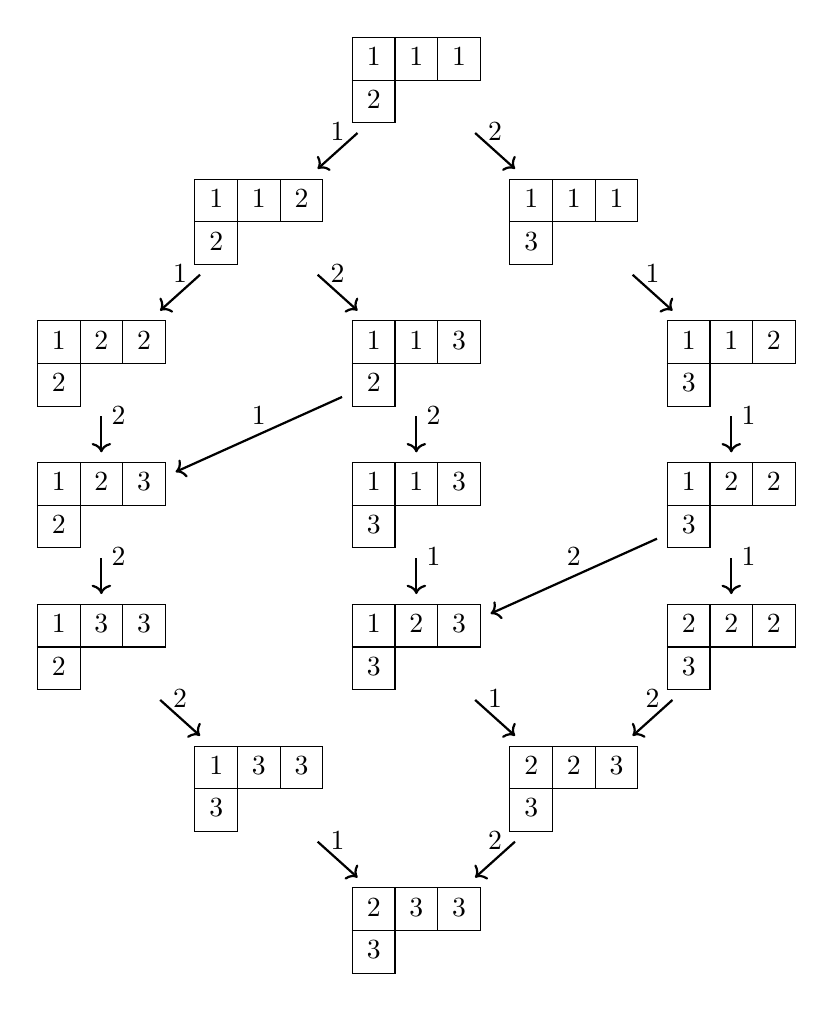
\begin{tikzpicture}
  \node (1) at (0, 0) {$\ytableaushort{111,2}$};
  
  \node (2) at (-2, -1.8) {$\ytableaushort{112,2}$};
  \node (3) at (2, -1.8) {$\ytableaushort{111,3}$};
  
  \node (4) at (-4, -3.6) {$\ytableaushort{122,2}$};
  \node (5) at (0, -3.6) {$\ytableaushort{113,2}$};
  \node (6) at (4, -3.6) {$\ytableaushort{112,3}$};
  
  \node (7) at (-4, -5.4) {$\ytableaushort{123,2}$};
  \node (8) at (0, -5.4) {$\ytableaushort{113,3}$};
  \node (9) at (4, -5.4) {$\ytableaushort{122,3}$};
  
  \node (10) at (-4 ,-7.2) {$\ytableaushort{133,2}$};
  \node (11) at (0, -7.2) {$\ytableaushort{123,3}$};
  \node (12) at (4, -7.2) {$\ytableaushort{222,3}$};
  
  \node (13) at (-2, -9) {$\ytableaushort{133,3}$};
  \node (14) at (2, -9) {$\ytableaushort{223,3}$};
  
  \node (15) at (0, -10.8) {$\ytableaushort{233,3}$};
  
  \draw[->, thick] (1) -- node[above] {$1$} (2);
  \draw[->, thick] (1) -- node[above] {$2$} (3);

  \draw[->, thick] (2) -- node[above] {$1$} (4);
  \draw[->, thick] (2) -- node[above] {$2$} (5);
  \draw[->, thick] (3) -- node[above] {$1$} (6);

  \draw[->, thick] (4) -- node[above right] {$2$} (7);
  \draw[->, thick] (5) -- node[above] {$1$} (7);
  \draw[->, thick] (5) -- node[above right] {$2$} (8);
  \draw[->, thick] (6) -- node[above right] {$1$} (9);
  
  \draw[->, thick] (7) -- node[above right] {$2$} (10);
  \draw[->, thick] (8) -- node[above right] {$1$} (11);
  \draw[->, thick] (9) -- node[above right] {$1$} (12);
  \draw[->, thick] (9) -- node[above] {$2$} (11);

  \draw[->, thick] (10) -- node[above] {$2$} (13);
  \draw[->, thick] (11) -- node[above] {$1$} (14);
  \draw[->, thick] (12) -- node[above] {$2$} (14);

  \draw[->, thick] (13) -- node[above] {$1$} (15);
  \draw[->, thick] (14) -- node[above] {$2$} (15);
\end{tikzpicture}

次に, $\mathcal{B}_{\lambda}$ が $\mathbb{B}^{ \otimes k}$ の連結成分であることを示すために
以下の写像を用意する.

\begin{df}
  写像 $RR : \mathcal{B}_{\lambda} \to \mathbb{B}^{ \otimes k}$ を次のように定める. 
  $T \in \mathcal{B}_{\lambda}$ の row word が
  $$\pi_T = i_1 i_2 \cdots i_k $$
  であるとき  
  \[
    RR (T) = 
    \begin{ytableau} i_1 \end{ytableau} \otimes 
    \begin{ytableau} i_2 \end{ytableau} \otimes 
    \cdots \otimes 
    \begin{ytableau} i_k \end{ytableau}
  \]
  とする. これを \text{row reading} という.
\end{df}

本論文では扱わないが, $\mathcal{B}_{\lambda}$ から $\mathbb{B}^{ \otimes k}$ への写像の定め方は
この row reading 以外に column reading と呼ばれるものなどもある.

\begin{ex}
  $T = \ytableaushort{23336, 347, 5}$ とする. このとき,
  $\pi_T = 5 3 4 7 2 3 3 3 6$ である. よって,
  \[
    RR(T) = 
    \begin{ytableau} 5 \end{ytableau} \otimes
    \begin{ytableau} 3 \end{ytableau} \otimes
    \begin{ytableau} 4 \end{ytableau} \otimes
    \begin{ytableau} 7 \end{ytableau} \otimes
    \begin{ytableau} 2 \end{ytableau} \otimes
    \begin{ytableau} 3 \end{ytableau} \otimes
    \begin{ytableau} 3 \end{ytableau} \otimes
    \begin{ytableau} 3 \end{ytableau} \otimes
    \begin{ytableau} 6 \end{ytableau}
  \]
  である.
\end{ex}

\begin{prop}[{\cite[命題3.1]{b2}}]
  写像 $RR$ は $\mathcal{B}_{\lambda}$ から $\mathbb{B}^{ \otimes k}$ への準同型である.
\end{prop}

\begin{proof}
  準同型の定義 (H1) から (H3) を満たすことを確認すれば良い.
  \begin{enumerate}
    \item[(H1)] (H1a) から (H1c) が成り立つことを確認する.
    \begin{enumerate}
      \item[(H1a)] 明らか. 
      \item[(H1b)] $\mathcal{B}_{\lambda}$ と $\mathbb{B}^{ \otimes k}$ が seminormal であることと後で示す (H2) から分かる.
      \item[(H1c)] $\mathcal{B}_{\lambda}$ と $\mathbb{B}^{ \otimes k}$ が seminormal であることと後で示す (H3) から分かる.
    \end{enumerate}
    \item[(H2)] $T \in \mathcal{B}_{\lambda}$ とし, $T$ の行を $T_1, T_2, \cdots, T_l$ とする.
    このとき, $RR(T) = RR(T_l) \otimes RR(T_{l-1}) \otimes \cdots \otimes RR(T_1)$ と表せる. $f_i$ を適応すると, 
    $$f_i(RR(T)) = RR(T_l) \otimes RR(T_{l-1}) \otimes \cdots \otimes f_i(RR(T_j)) \otimes \cdots \otimes RR(T_1)$$
    ( ただし, $j$ は, $\sum_{h \geq j } \varphi_i(RR(T_h)) - \sum_{ h > j } \varepsilon_i (RR(T_h))$ を満たす $l$ 以下の最大の正整数. )
    となる. $T'$ を $T_1, T_2, \cdots, f_i(T_j), \cdots, T_l$ を行に持つ tableau とする. $T'$ が semistandard であれば,
    $f_i(RR(T)) = RR(T') = RR(f_i(T))$ であることを導ける. $T'$ が semistandard でないとすると, $T_j$ で $i$ が $i + 1$ に
    変わった成分の下にある成分が $i + 1$ である. $T$ は seminormal であるから, $j$ 行目の $i$ がある成分の下にある $j + 1$ 行目の
    成分は $i + 1$ になる. よって, $\varepsilon_i(T_{j + 1}) \geq \varphi_i(T_j)$ である.
    これは, $j$ が $\sum_{h \geq j } \varphi_i(RR(R_h)) - \sum_{ h > j } \varepsilon_i (RR(R_h))$
    が最大となるときであることに矛盾する.
    \item[(H3)] (H2) と同様に示せば良い.
  \end{enumerate}
\end{proof}

連結な crystal の特徴を探るため, 次を定義する.

\begin{df}
  任意の $i \in I$ で $e_i(u) = 0$ となる元 $u \in \mathcal{B}$ を最高 weight 元という. このとき, $\mathrm{wt}(u)$ を最高 weightという.
\end{df}

$\mathcal{B}_{\lambda}$ や $\mathbb{B}^{\otimes k}$ は有限集合より, 最高 weight 元が存在することが分かる.

\begin{ex}
  $\mathbb{B}$ の 最高 weight 元 は $\ytableaushort{1}$ , 最高 weight は $1$ である.
\end{ex}

\begin{df}
  $i$ 行の成分が全て $i$ である形 $\lambda$ のsemistandard tableau を $u_\lambda$ で表す.
\end{df}

\begin{ex}
  $\lambda= (4, 2)$ であるとき, $u_\lambda = \ytableaushort{1111,22}$ である.
\end{ex}

最高 weight 元の概念を用いて, $\mathcal{B}_{\lambda}$ が連結な crystal であることを示す.

最高 weight 元が一意性であれば
その crystal の任意の元は 最高 weight 元 に $f_i$ を有限回適応することで
表せることができる.
しかし, 最高 weight 元が一意性でなければ, 最高 weight 元は他の最高 weight 元に
Kashiwara 作用素を有限回適応することで表せることができないため, 連結ではないことが分かる.
これを利用して, crystal の連結性を示していくのである.

\begin{thm}[{\cite[定理3.2]{b2}}] \label{crystal-of-tableau}
  $\lambda$ を長さは $n$ 以下の $k$ の分割とする.
  このとき, $RR(\mathcal{B}_{\lambda})$ は, $\mathbb{B}^{\otimes k}$ の連結成分になる.
  さらに, 一意的な最高 weight 元 $RR(u_\lambda)$ を持つ.
\end{thm}

\begin{proof}
  命題3より, $RR(u_\lambda)$ が一意的な最高 weight 元であることを示せば, $\mathbb{B}^{\otimes k}$ の連結成分であることが分かる.
  $T \in \mathcal{B}_{\lambda}$ を最高 weight 元とし, $T$ の行を $T_1, T_2, \cdots, T_l$ とする.
  $e_i(RR(T)) = 0$ より, $\varepsilon_i(RR(T)) = 0$ である. よって,
  $$\varepsilon_i(T_1) = 0, \quad \varepsilon_i(T_1) + \varepsilon_i(T_2) - \varphi_i(T_1) \leq 0, \quad  \cdots $$
  である. $\varepsilon_i(T_1) = 0$ より, $T_1$ の成分は $1$ のみであることが分かる.
  $\varepsilon_i(T_2) - \varphi_i(T_1) \leq 0$ より, $i > 1$ であるならば, $\varepsilon_i(T_2) = 0$ より,
  $T_2$ の成分は $1, 2$ である. $T$ は seminormal より, $T_2$ の成分は $2$ のみである.
  $T_3, T_4 \cdots$ も同様に考えれば, $T = u_\lambda$ であることが分かる.
\end{proof}

次に, $\mathbb{B}^{ \otimes k}$ を連結な crystal の直和分解をすると,
どうなるかを議論するために, いくつかの補題を用意する.
crystal $\mathcal{B}$ の subcrystal とは, $\mathcal{B}$
の部分集合で crystal であるものを指す.

\begin{lem}[{\cite[命題2.16]{b2}}] \label{higest-weight-is-partation}
  $\mathbb{B}^{ \otimes k}$ の subcrystal の 最高 weight は,
  分割である.
\end{lem}

\begin{proof}
  $\mathcal{B}$ を $\mathbb{B}^{ \otimes k}$ の subcrystal とする.
  $u$ を $\mathcal{B}$ の 最高 weight 元とする.
  このとき, $\varepsilon_i(u) = 0$ より,
  $\langle \mathrm{wt}(u), \alpha_i^{ \vee } \rangle = \varphi_i(u) \geq 0$ である.
  $\mathrm{wt}(u) = (\lambda_1, \cdots, \lambda_n )$ とすると,
  $ 0 \leq \langle \mathrm{wt}(u), \alpha_i^{ \vee } \rangle = \lambda_i - \lambda_{ i + 1}$
  である. よって, $\lambda_i \leq \lambda_{ i + 1 }$ と $i$ の任意性から, $\mathrm{wt}(u)$
  は分割である.
\end{proof}

\begin{lem}{\cite[定理4.11]{b2}}
  $x \in \mathbb{B}^{ \otimes k} , i \neq j, f_i x, f_j x \neq 0$ とする. このとき,
  \begin{enumerate}
    \item
    $| i - j | \neq 1$ のとき, 
    $$f_if_j x =f_jf_i x \neq 0$$
    が成り立つ.
    このとき,
    $$\varphi_j(f_ix) = \varphi_j(x), \quad \varphi_i(f_jx) = \varphi_i(x)$$
    が成り立つ.
    \item
    $| i - j | = 1$ のとき,
    $$f_if_j x = f_jf_i x \neq 0$$ 
    または
    $$f_if_j^2f_i x = f_jf_i^2f_j x \neq 0$$
    のいずれかが成り立つ.
    前者が成り立つとき,
    $$\varphi_j(f_ix) = \varphi_j(x), \quad \varphi_i(f_jx) = \varphi_i(x) + 1$$
    または
    $$\varphi_j(f_ix) + 1 = \varphi_j(x), \quad \varphi_i(f_jx) = \varphi_i(x)$$
    が成り立つ.
    後者が成り立つとき,
    $$\varphi_j(f_ix) + 1 = \varphi_j(x), \quad \varphi_i(f_jx) = \varphi_i(x) + 1$$
    が成り立つ.
  \end{enumerate}
\end{lem}

\begin{proof}
  signature rule を利用して考える.

  $| i - j | \neq 1$ とする.
  $i, i + 1, j, j + 1$ の全ての値が異なるから,
  $f_i x$ と $x$ の $j, j + 1$ のあり方は変わらない. よって,
  $f_jf_i x$ と $f_jx$ の $j, j + 1$ のあり方は変わらない. よって,
  $f_jf_i x$ と $f_if_jx$ の $j, j + 1$ のあり方は変わらない.
  同様に, $f_jf_i x$ と $f_if_jx$ の $i, i + 1$ のあり方は変わらない.
  よって, $f_if_j x = f_jf_i x$ である.
  また, $\varphi_j(f_ix) = \varphi_j(x), \varphi_i(f_jx) = \varphi_i(x)$
  が成り立つ.

  次に $j = i + 1$ とする. ($i = j - 1$ も同様に示せる. )
  $f_ix$ に $f_{i + 1}$ を適応すると, $f_ix$ で $i$ が $i + 1$ に変わった場所 $t_1$ で $i + 1$ が $i + 2$ になる可能性がある.
  そうであるとき, $f_{i + 1}f_ix$ に  $f_{i + 1}$ を適応すると, $t$ より前で $i + 1$ が $i + 2$ になる. この場所を
  $t_2$ とする. この $f_{i + 1}^2f_ix$ に $f_i$ を適応すると,
  $t_2$ にあった $i + 1$ の括弧のペアだった $i$ が括弧がなくなる. 
  したがって, $t_2$ から $t_1$の間に $i$ が少なくとも1つはあり, その間で $i$ が $i + 1$ になる.
  このとき, $\varphi_j(f_{i}x) = \varphi_j(x) + 1$ である.
  この状況の下, 右辺を考える.
  $x$ に $f_j$ を適応すると, $t_2$ で $i + 1$ が $i + 2$ になる.
  $f_jx$ に $f_i$ を適応すると, $t_1$ で $i$ が $i + 1$ になる.
  $f_if_jx$ に $f_i$ を適応すると, $t_2$ から $t_1$の間にある $i$ が $i + 1$ になる.
  $f_i^2f_jx$ に $f_j$ を適応すると, $t_1$ で $i + 1$ が $i + 2$ となる.
  したがって, $f_if_j^2f_i x = f_jf_i^2f_j x$ となる.
  ( $f_if_jx$ に $f_j$ を適応すると, $t_2$ にある $i + 2$ と $t$ にある $i +1$ で括弧がくくれる可能性があり,
  $t_1$ で $i + 2$ にならない可能性がある. )
  このとき, $\varphi_i(f_{j}x) = \varphi_i(x) + 1$ である.

  他の場合として, $f_jx$ に $f_i$ を適応すると, $x$ から $f_jx$ で変わった $i + 1$ のペアだった $i$ が $i + 1$
  になる可能性がある. この場合も同様に考えれば良い.

  それ以外の場合は, $f_if_j x = f_jf_i x$ となる.
  この場合, $f_{j}x$ で $i + 1$ から $i + 2$ に変わった場所は, $i + 1$ と $i$ のペアで括弧がくくっていない場所である.
  実際, 括弧がくくってあるとすると, この括弧より右側に括弧がくくっていない $i$ があるときは, 最初に述べたケースになる.
  右側に括弧がくくっていない $i$ がないときは, その次に述べたケースになるからである.
  よって, $\varphi_i(f_jx) = \varphi_i(x)$ である. $\varphi_j(f_ix) = \varphi_j(x) + 1$ であることは
  $f_ix$ で $i + 1$ が一つ増えたことから言える.
\end{proof}

上記と同様に考えることで, $e_i$ に関しても同様のことが言える.

\begin{lem}{\cite[定理4.11]{b2}} \label{stembridge}
  $x \in \mathbb{B}^{ \otimes k} , i \neq j, e_i x, e_j x \neq 0$ とする. このとき,
  \begin{enumerate}
    \item
    $| i - j | \neq 1$ のとき, 
    $$e_ie_j x =e_je_i x \neq 0$$
    が成り立つ.
    このとき,
    $$\varepsilon_j(e_i(x)) = \varepsilon_j(x), \quad \varepsilon_i(e_j(x)) = \varepsilon_i(x)$$
    が成り立つ.
    \item
    $| i - j | = 1$ のとき,
    $$e_ie_j x =e_je_i x \neq 0$$ 
    または
    $$e_ie_j^2e_i x = e_je_i^2e_j x \neq 0$$
    のいずれかかが成り立つ.
    前者が成り立つとき,
    $$\varepsilon_j(e_i(x)) = \varepsilon_j(x), \quad \varepsilon_i(e_j(x)) = \varepsilon_i(x) + 1$$
    または
    $$\varepsilon_j(e_i(x)) + 1 = \varepsilon_j(x), \quad \varepsilon_i(e_j(x)) = \varepsilon_i(x)$$
    が成り立つ.
    後者が成り立つとき,
    $$\varepsilon_j(e_i(x)) + 1 = \varepsilon_j(x), \quad \varepsilon_i(e_j(x)) = \varepsilon_i(x) + 1$$
    が成り立つ.
  \end{enumerate}
\end{lem}

これを用いると, 以下の定理が言える.
この証明では, 次の $\mathrm{rank}$ という概念を利用する.

crystal $\mathcal{B}$ の 元 $x$ に対して,
$\mathcal{B}$ の中にある最高 weight 元 $u$ を用いて, 
\[
u = e_{i_N} \cdots e_{i_2} e_{i_1} x
\]
が成り立つとする. このとき, 作用素の適用回数 $N$ を $\mathrm{rank}(x)$ とする.

\begin{thm} [{\cite[定理4.12, 定理4.13, 系6.2]{b2}}] \label{direct-sum-decomposition}
  \begin{enumerate}
    \item[]
    \item 連結な $\mathbb{B}^{ \otimes k}$ の subcrystal は, 一意的な最高 weight 元を持つ.
    \item 2つの連結な $\mathbb{B}^{ \otimes k}$ の subcrystal の 最高 weight が等しいとき, この2つの subcrystal は同型である.
    \item 連結な $\mathbb{B}^{ \otimes k}$ の subcrystal は ある $\mathcal{B}_{\lambda} ( \lambda \vdash n )$ に同型である.
  \end{enumerate}
\end{thm}

\begin{proof}
  $\mathcal{B}$, $\mathcal{B}'$ を連結な $\mathbb{B}^{ \otimes k}$ の subcrystal とする.
  \begin{enumerate}
    \item
    crystal $\mathcal{B}$ 上に順序 $x \geq y$ を次のように定める.  
    ある列 $i_1, \dots, i_m$ が存在して,
    \[
    x = e_{i_1} \cdots e_{i_m} y
    \]
    と表せるとき, $x \geq y$ とする.

    $\mathcal{B}$ は有限集合より, 極大元 $x$ が存在する.
    $\Omega = \{ y \in \mathcal{B} \mid y \leq x \}$ とする.
    $S \neq \emptyset$ とする.
    $S$ を $y \in \Omega, 0 \neq e_i y \notin \Omega$ なる元全体とすると,
    $S \neq \emptyset$ である.
    $y$ を $S$ の極大元とする.
    $e_i y \notin \Omega$ より, $y$ は最高 weight 元でない.
    $y \leq x$ より, ある $j$ で $0 \neq e_j(y) \in \Omega$ である.
    補題 \ref{stembridge} より, $e_ie_j(y) = e_je_i(y) \neq 0$ または
    $e_ie_j^2e_i = e_je_i^2e_j \neq 0$ のいずれかが成り立つ.
    まず, 前者を考える.
    $y$ の極大性より, $e_jy \notin S$ となる.
    よって, $e_ie_jy \in \Omega$ である.
    よって, $e_iy \leq e_je_iy = e_ie_jy \leq x$ となり, $e_iy \notin \Omega$ に矛盾する.
    次に後者を考える.
    前者と同様に, $e_jy \notin S$ である.
    $e_ie_jy \geq y$ より, $e_ie_jy \notin S$ であるから,
    $e_i^2e_jy \in \Omega$ である.
    さらに, $e_i^2e_jy\geq y$ より, $e_i^2e_jy \notin S$ であるから,
    $e_je_i^2e_jy \in \Omega$ である.
    よって, $e_iy \leq e_ie_j^2e_iy = e_je_i^2e_jy \leq x$ となり, $e_iy \notin \Omega$ に矛盾する.
    以上より, $S = \emptyset$ であることが分かる.

    次に, $\mathcal{B} \backslash \Omega = \emptyset$ でないと仮定する.
    $z \in \mathcal{B} \backslash \Omega$ で, $z = f_iy$ または $z = e_iy$ となる元が存在する.
    1番目は, $z \leq y \leq x$, $z \notin \Omega$ に矛盾する.
    2番目は, $S = \emptyset$ に矛盾する.
    以上より, $\mathcal{B} = \Omega$ を示せた.
    \item 
    $u, u'$ を $\mathcal{B}$, $\mathcal{B}'$ の最高 weight 元とする.
    $\Omega$ を次を満たす $\mathcal{B}$ の部分集合 $S$ とする.
    \begin{enumerate}
      \item $u \in S$
      \item $x \in S, e_ix \neq 0$ のとき, $e_ix \in S$.
      \item $\mathcal{B}'$ の部分集合 $S'$ が存在して,
      $S$ から $S'$ への全単射な写像で $u$ が $u'$ に値をもつものが存在する.
      このとき, $x \in S$ のこの写像での値を $x'$ で表す.
      さらに, $e_ix \neq 0$ と $e_ix' \neq 0$ 
      が必要十分条件となる. また, $(e_ix)' = e_i x'$ が成り立つ.
    \end{enumerate}
    $\{ u \} \in \Omega$ より, $\Omega$ は空ではない.
    $S$ を 包含関係に関して極大な $\Omega$ の元とする.

    始めに, $\mathrm{wt}(x) = \mathrm{wt}(x'), \varepsilon_i(x) = \varepsilon_i(x'),
    \varphi_i(x) = \varphi_i(x')$ を示す.
    $N = \mathrm{rank}(x)$ であるならば, $u = e_{i_N} \cdots e_{i_2}e_{i_1} x$ となるものがある.
    $e_{i_N} \cdots e_{i_2}e_{i_1} x' = (e_{i_N} \cdots e_{i_2}e_{i_1} x)' = u'$ である.
    よって, 
    $
    \mathrm{wt}(x') = \mathrm{wt}(u') - \sum_{j = 1}^{N} \alpha_{i_j}
    = \mathrm{wt}(u) - \sum_{j = 1}^{N} \alpha_{i_j} = \mathrm{wt}(x)
    $
    となる. \\
    次に, $\varepsilon_i(x)$ を $e_i^k x \neq 0$ となる 最大の数 $k$ とする.
    このとき, $e_i^kx' = (e_i^kx)' \neq 0$, $e_i^{k + 1}x' = (e_i^{k + 1}x)' = 0$
    より, $\varepsilon_i(x')$ も $k$ になるから, $\varepsilon_i(x) = \varepsilon_i(x')$ となる.
    最後に, $\varphi_i(x) = \langle \mathrm{wt}(x), \alpha_i \rangle - \varepsilon_i(x)$
    から, $\varphi_i(x) = \varphi_i(x')$ が分かる.

    最後に$S = \mathcal{B}$ を示す. $S \neq \mathcal{B}$ とする.
    $ z \in \mathcal{B} \backslash S$ を $\mathrm{rank}$ に関して極小な元とする.
    $z \neq u$ より, $e_iz \neq 0$ となる $i$ がある.
    $\mathrm{rank}(e_iz) < \mathrm{rank}(z)$ と $z$ の極小性より, $e_iz \in S$ である.
    $\varphi_i((e_iz)') = \varphi_i((e_iz)) \neq 0$ であるから,
    $e_i \tilde{z} = (e_iz)'$ となる $\tilde{z} \in \mathcal{B}'$ がある.
    この $\tilde{z}$ が $i$ によらないことを示す.
    即ち, $e_jz \neq 0$ となる $j$ に対し, $e_j \bar{z} = \bar{e_jz}$ となる
    $ \bar{z} \in \mathcal{B}'$ がある. このとき, $\tilde{z} = \bar{z}$ を示す.
    $e_i z, e_j z \neq 0$ であるから, 補題 \ref{stembridge} より,
    $e_ie_j z = e_je_i z \neq 0$ か $e_je_i^2e_j z = e_ie_j^2e_i z \neq 0$
    のいずれかが成り立つ.
    1番目の状況では $w = e_ie_j z$, 2番目の状況では $w = e_je_i^2e_j z$ とする.
    $e_i z, e_j z \in S$ と $S$ の定め方から, $w, f_iw, f_jw \in S$ である.
    よって, 
    $\varphi_i(w') = \varphi_i(w'), \varphi_i(f_jw') = \varphi_i((f_jw)') = \varphi_i(f_jw),
    \varphi_j(f_iw') = \varphi_j((f_jw)') = \varphi_j(f_iw)$
    が成り立つ.
    よって, $w', f_iw', f_jw' \neq 0$ であるから,
    1番目は $f_if_jw' = f_jf_iw'$, 2番目は $f_if_j^2f_iw' = f_jf_i^2f_jw'$
    が成り立つ.

    1番目は $f_jw = e_iz$ より, $e_i \tilde{z} = (e_iz)' = (f_jw)' = f_jw'$ であるから,
    $w' = e_je_i \tilde{z}$ である. 同様に, $w' = e_je_i \bar{z}$ である.
    よって, $\tilde{z} = f_if_jw' = f_jf_iw' = \bar{z}$ となる.

    2番目は $e_ie_je_iw = z$ であるから, 
    $e_i \tilde{z} = (e_iz)' = (f_j^2f_iw)' = f_j^2f_iw'$ である.
    同様に, $e_i \bar{z} = f_j^2f_iw'$ である.
    よって, $\tilde{z} = \bar{z}$ である.

    $S \cup \{ z \}$ から $S' \cup \{ z' \}$ への写像を $x \in S$ を $x' \in S'$ へ,
    $z$ を $z'$ へ写すとすると, これは well-defined. よって, $S$ の極大性に矛盾する.
    よって, $S = \mathcal{B}$ となる. $\mathcal{B}'$ から $\mathcal{B}$ への逆写像も同様に存在する.
    \item $\mathcal{B}$ は一意的な最高 weight 元が存在する.
    その weight を $\lambda$ とする.
    補題 \ref{higest-weight-is-partation} より, $\lambda$ は分割である.
    定理 \ref{crystal-of-tableau} と この定理の2より, 分かる.
  \end{enumerate}
\end{proof}

この定理より, 連結な $\mathbb{B}^{ \otimes k}$ の subcrystal と
それに対応する $\mathcal{B}_{\lambda}$ を同一視する.
また, $\mathbb{B}^{ \otimes k}$ 内の 連結な subcrystal の個数と
最高 weight 元の個数が一致することが分かる.

具体的に $\mathbb{B}^{ \otimes 3}$ を直和分解してみる.
そのために, 最高 weight 元 であることを判別するために
Yamanouchi word を定義する.
$\mathbb{B}^{ \otimes 3}$ を直和分解は, 次の節の plactically 同値と RSK 対応の関係に関する定理の
証明の際に利用する.

\begin{df}
  \begin{enumerate}
    \item[]
    \item 
    $x =     
    \begin{ytableau} i_1 \end{ytableau} \otimes 
    \begin{ytableau} i_2 \end{ytableau} \otimes 
    \cdots \otimes 
    \begin{ytableau} i_k \end{ytableau}
    \in \mathbb{B}^{ \otimes k}
    $
    とする. $x$ の reading word を
    $$ \operatorname{word}(x) = i_1 i_2 \cdots i_k $$
    とする.
    \item word $i_1 i_2 \cdots i_k$ が Yamanouchi word であるとは, 
    任意の終端セグメント $ \{ i_j \cdots i_k \} $ と任意の $i$ に対して, 
    $i + 1$ の数が $i$ の数以下であるときをいう.
  \end{enumerate}
\end{df}

\begin{ex}
  \[
    x = \ytableaushort{2} \otimes \ytableaushort{3} \otimes \ytableaushort{2} \otimes \ytableaushort{1} \otimes \ytableaushort{1}
    \in \mathbb{B}^{\otimes 5}
  \]
  とする.
  このとき,
  \[
    \operatorname{word}(x) = 2 3 2 1 1
  \]
  である. この word は Yamanouchi word である.

  実際, 終端セグメント $\{ 1\}, \{ 1 1\}, \{ 2 1 1\}, \{ 3 2 1 1\}, \{ 2 3 2 1 1\}$ と 任意の $i$ に対して,
  それぞれ $i + 1$ が $i$ 以下である.
\end{ex}

\begin{prop} [{\cite[命題8.2]{b2}}]
  $x =     
  \begin{ytableau} i_1 \end{ytableau} \otimes 
  \begin{ytableau} i_2 \end{ytableau} \otimes 
  \cdots \otimes 
  \begin{ytableau} i_k \end{ytableau}
  \in \mathbb{B}^{ \otimes k}
  $ 
  が最高 weight 元であることと $\operatorname{word}(x)$ が Yamanouchi word
  であることは必要十分条件である.
\end{prop}

\begin{proof}
  対偶で示す. 命題 \ref{crystal-tensor} より,
  $$
  \varepsilon_i(x) = \max_{j = 1}^{k} \left( \sum_{h = j}^{k} \varepsilon_i(i_h) - \sum_{h = j + 1}^{k} \varphi_i(i_h) \right)
  $$
  である.
  また, $\varepsilon_i$ は, ${\begin{ytableau} \scriptstyle{i + 1} \end{ytableau}}$ のとき $1$, それ以外は $0$ である.
  よって, $\max$ が $0$ でないならば, $i_j = j + 1$ のとき, 最大になる. このとき, $\varepsilon_i(i_j) = 0$ であるから,
  $$\varepsilon_i(x) = \max_{j = 1}^{k}\left(  \sum_{h = j}^{k} (\varepsilon_i(i_h) - \varphi_i(i_h)) \right)$$
  と表せる. $\varepsilon_i - \varphi_i$ は, ${\begin{ytableau} \scriptstyle{i + 1} \end{ytableau}}$ のとき $1$, 
  ${\begin{ytableau} i \end{ytableau}}$ のとき $-1$, それ以外は $0$ だから, max が $0$ でないならば, ある $j$ で, 
  ${i_j, i_{j + 1}, \cdots, i_k}$ で $i$ の数より $i + 1$ の数が大きい必要がある. よって, $\operatorname{word}(x)$
  は Yamanouchi word ではない. 逆に,  $\operatorname{word}(x)$ が Yamanouchi word ではないとき, ある $j$ で, 
  ${i_j, i_{j + 1}, \cdots, i_k}$ で $i$ の数より $i + 1$ の数が大きい. このとき, $\max$ 内で この $j$ で $0$ ではない.
  よって, $x$ は最高 weight 元ではない.
\end{proof}

\begin{prop} [{\cite[命題8.3]{b2}}]
  $n \geq 3$ とする.
  このとき, $\mathbb{B}^{ \otimes 3}$ は $\mathcal{B}_{(3)} \oplus \mathcal{B}_{(2, 1)} \oplus \mathcal{B}_{(2, 1)} \oplus \mathcal{B}_{(1^3)}$ 
  に同型である.
\end{prop}

\begin{proof}
  $x = \ytableaushort{p} \otimes \ytableaushort{q} \otimes \ytableaushort{r} \in \mathbb{B}^{\otimes 3}$ 
  の row word が Yamanouchi word となるときを考える.
  $\operatorname{word}(x) = p q r$ より, 終端セグメント ${r}$ を考えると, $r = 1$.
  終端セグメント ${q, r}$ を考えると, $q = 1, 2$.
  終端セグメント ${p, q, r}$ を考えると, $q = 1$ ならば $r = 1, 2$, $q = 2$ ならば $r = 1, 3$.
  よって, 
  $$
  x = 
  \ytableaushort{1} \otimes \ytableaushort{1} \otimes \ytableaushort{1}, \quad
  \ytableaushort{2} \otimes \ytableaushort{1} \otimes \ytableaushort{1}, \quad
  \ytableaushort{1} \otimes \ytableaushort{2} \otimes \ytableaushort{1}, \quad
  \ytableaushort{3} \otimes \ytableaushort{2} \otimes \ytableaushort{1}
  $$
  である. weight を考えれば, $(3), (2, 1), (2, 1), (1^3)$ より分かる.
\end{proof}

$\mathcal{B}_{(2, 1)}$ に同型な2つの crystal を区別するために,
最高 weight 元 が $\ytableaushort{1} \otimes \ytableaushort{2} \otimes \ytableaushort{1}$ を持つ $\mathcal{B}_{(2, 1)}$
に同型な crystal を $\mathcal{B}'_{(2, 1)}$ で表すことにする.

また, この同型において
$\ytableaushort{1} \otimes \ytableaushort{1} \otimes \ytableaushort{1} \in \mathbb{B}^{\otimes 3}$ 
は $\ytableaushort{111} \in \mathcal{B}_{(3)}$ に対応している.

同様に, $\ytableaushort{2} \otimes \ytableaushort{1} \otimes \ytableaushort{1}$ および $\ytableaushort{1} \otimes \ytableaushort{2} \otimes \ytableaushort{1}$ 
はそれぞれ $\ytableaushort{11,2}$ に, $\ytableaushort{3} \otimes \ytableaushort{2} \otimes \ytableaushort{1}$ は $\ytableaushort{1,2,3}$ に対応している.

\begin{ex}
  $n = 3$ とする.
  例えば $\mathcal{B}_{(3)}$ に対応する $\mathbb{B}^{ \otimes 3}$ の subcrystal を記述すると, 以下のようになる.
\end{ex}
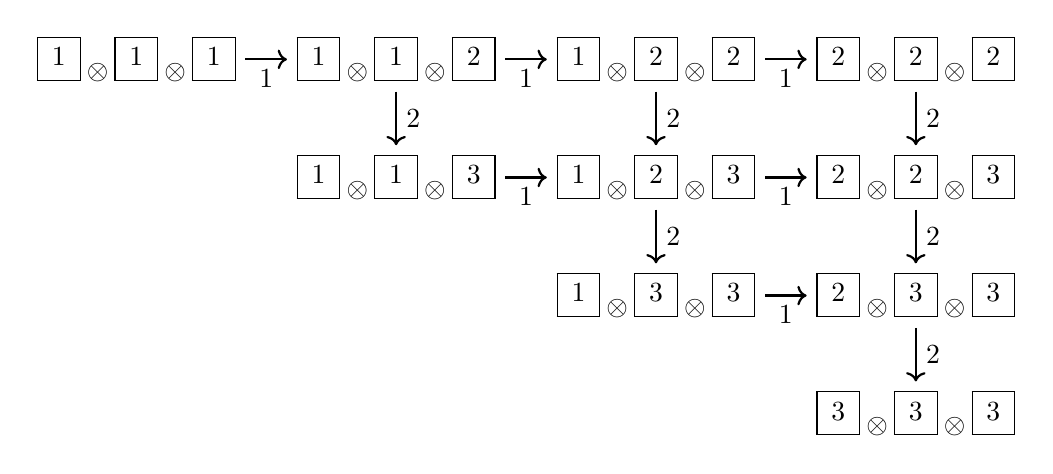
\begin{tikzpicture}
  \node (11) at (0, 0) {\(\ytableaushort{1} \otimes \ytableaushort{1} \otimes \ytableaushort{1}\)};
  \node (12) at (3.3, 0) {\(\ytableaushort{1} \otimes \ytableaushort{1} \otimes \ytableaushort{2}\)};
  \node (13) at (6.6, 0) {\(\ytableaushort{1} \otimes \ytableaushort{2} \otimes \ytableaushort{2}\)};
  \node (14) at (9.9,0) {\(\ytableaushort{2} \otimes \ytableaushort{2} \otimes \ytableaushort{2}\)};
  
  \node (21) at (3.3, -1.5) {\(\ytableaushort{1} \otimes \ytableaushort{1} \otimes \ytableaushort{3}\)};
  \node (22) at (6.6, -1.5) {\(\ytableaushort{1} \otimes \ytableaushort{2} \otimes \ytableaushort{3}\)};
  \node (23) at (9.9, -1.5) {\(\ytableaushort{2} \otimes \ytableaushort{2} \otimes \ytableaushort{3}\)};
  
  \node (31) at (6.6, -3) {\(\ytableaushort{1} \otimes \ytableaushort{3} \otimes \ytableaushort{3}\)};
  \node (32) at (9.9, -3) {\(\ytableaushort{2} \otimes \ytableaushort{3} \otimes \ytableaushort{3}\)};

  \node (41) at (9.9, -4.5) {\(\ytableaushort{3} \otimes \ytableaushort{3} \otimes \ytableaushort{3}\)};
  
  \draw[->, thick] (11) -- node[below]{$1$} (12);
  \draw[->, thick] (12) -- node[below]{$1$} (13);
  \draw[->, thick] (13) -- node[below]{$1$} (14);
  \draw[->, thick] (12) -- node[right]{$2$} (21);
  \draw[->, thick] (13) -- node[right]{$2$} (22);
  \draw[->, thick] (14) -- node[right]{$2$} (23);

  \draw[->, thick] (21) -- node[below]{$1$} (22);
  \draw[->, thick] (22) -- node[below]{$1$} (23);
  \draw[->, thick] (22) -- node[right]{$2$} (31);
  \draw[->, thick] (23) -- node[right]{$2$} (32);

  \draw[->, thick] (31) -- node[below]{$1$} (32);
  \draw[->, thick] (32) -- node[right]{$2$} (41);
\end{tikzpicture}

写像 $RR$ において $RR \left(\ytableaushort{11,2} \right) = \ytableaushort{2} \otimes \ytableaushort{1} \otimes \ytableaushort{1}$ である. 
しかし, $RR(x) = \ytableaushort{1} \otimes \ytableaushort{2} \otimes \ytableaushort{1}$ となる tableau のcrystal の元 $x$ は存在しない.

$RR$ は tableau のcrystal を $\mathbb{B}^{\otimes k}$ へ写す写像である. 
逆に, $\mathbb{B}^{\otimes k}$ を tableau のcrystal へ写す写像は, 
$\mathbb{B}^{\otimes k}$ を tableau のcrystal の直和に分解した際に重複が生じるため, $RR$ の逆写像として実現できない.

そこで, 以降の説明するように P-tableau がその役割を果たすのである.

\subsection{plactically 同値と Knuth 同値}
次のセクションのため, plactically 同値と Knuth 同値 の関係性をここでは述べる.

\begin{df}
  $\mathcal{B}_1$, $\mathcal{B}_2$ を $A_r$ 型の crystal とする.
  $x_i \in \mathcal{B}_i$ とする.
  $x_1$ と $x_2$ がplactically 同値であるとは,
  \begin{enumerate}
    \item $\mathcal{B}_1 '$ と $\mathcal{B}_2 '$ が同型となる $x_i \in \mathcal{B}_i$ を含む連結成分 $\mathcal{B}_i '$ がある.
    \item crystal 同型写像 $\mathcal{B}_1 ' \to \mathcal{B}_2 '$ で $x_1 \mapsto x_2$ となるものがただ1つ存在する.
  \end{enumerate}
  を満たすときをいう. このとき, $x_1 \equiv x_2$ で表す.
\end{df}

\begin{thm} [{\cite[定理8.4]{b2}}] \label{k-plactically-equiv}
  $x, y \in \mathbb{B}^{\otimes k}$ とする.
  $\operatorname{word}(x) \equiv_{K} \operatorname{word}(y)$ であるならば, $x \equiv y$ である.
\end{thm}

\begin{proof}
  まず $k = 3$ の場合で示す. $\mathbb{B}^{\otimes 3} = \mathcal{B}_{(1^3)} \oplus \mathcal{B}^{'}_{(2, 1)} \oplus \mathcal{B}_{(2, 1)} \oplus \mathcal{B}_{(3)}$
  である. $a \leq b < c$ のとき,
  $x = \begin{ytableau} c \end{ytableau} \otimes \begin{ytableau} a \end{ytableau} \otimes \begin{ytableau} b \end{ytableau} \in \mathbb{B}^{\otimes 3}$
  と $y = \begin{ytableau} a \end{ytableau} \otimes \begin{ytableau} c \end{ytableau} \otimes \begin{ytableau} b \end{ytableau} \in \mathbb{B}^{\otimes 3}$
  が plactically 同値であることを示す. (もう一方の Knuth 同値である状況のときも以下と同様に示せる. ) このとき,
  $x$ は $\mathcal{B}_{(2, 1)}$, $y$ は $\mathcal{B}^{'}_{(2, 1)}$ と同一視できる.
  $\theta: \mathcal{B}_{(2, 1)} \to \mathcal{B}^{'}_{(2, 1)}$ を一意的な crystal 写像とする.
  このとき, $\theta(x) = y$ であることを示せばよい. $a$ を固定し, $b$ に関する帰納法で示す.

  $b = a$ のとき, $x, y$ の weight は等しく, $x, y$ は その weight を持つ$\mathcal{B}_{(2, 1)}, \mathcal{B}^{'}_{(2, 1)}$ の一意的な元だから,
  $\theta(x) = y$ であることが分かる. 次に, $a < b$ とし, 
  $x_1 = \begin{ytableau} c \end{ytableau} \otimes \begin{ytableau} a \end{ytableau} \otimes \begin{ytableau} \scriptstyle{ b - 1 } \end{ytableau}$,
  $y_1 = \begin{ytableau} a \end{ytableau} \otimes \begin{ytableau} c \end{ytableau} \otimes \begin{ytableau} \scriptstyle{ b - 1 } \end{ytableau}$
  で, $\theta(x_1) = y_1$ が成り立つと仮定する.
  $b < c$ より, $\varepsilon_{ b - 1 } c = 0$ である. $\varphi_{ b - 1 } (\begin{ytableau} a \end{ytableau} \otimes \begin{ytableau} \scriptstyle{ b - 1 } \end{ytableau}) \geq 1$ より,
  $f_{ b - 1 } x_1 = \begin{ytableau} c \end{ytableau} \otimes f_{ b - 1 } \begin{ytableau} a & \scriptstyle{ b - 1 } \end{ytableau} 
  = \begin{ytableau} c \end{ytableau} \otimes \begin{ytableau} a & b \end{ytableau} = x$ となる.
  同様に, $f_{ b - 1 } y_1 = y$ となる.
  よって, $\theta(x) = \theta (f_{ b - 1} x_1 ) = f_{ b - 1 } \theta(x_1) = f_{ b - 1 } y_1 = y$ である. これで, $k = 3$ のとき, 命題が成り立つことを示せた.
  $k \geq 3$ の場合, $x = u \otimes x_1 \otimes v, y = u \otimes y_1 \otimes v$ で,
  $x_1, y_1 \in \mathbb{B}^{\otimes 3}$ で $\operatorname{word}(x_1) \equiv_{K} \operatorname{word}(y_1)$,
  $u \in \mathbb{B}^{\otimes l}, v \in \mathbb{B}^{\otimes m}, l + m + 3 = k$ とする.
  このとき, 上記より, crystal $\mathcal{C}, \mathcal{D}, x_1 \in \mathcal{C}, y_1 \in \mathcal{D}$ で, $\mathcal{C}, \mathcal{D}$ が同型となるものが存在する.
  このとき, $\mathbb{B}^{\otimes l} \otimes \mathcal{C} \otimes \mathbb{B}^{\otimes m}, \mathbb{B}^{\otimes l} \otimes \mathcal{D} \otimes \mathbb{B}^{\otimes m}$
  は $x$ を $y$ にとる同型を誘導する. 
\end{proof}

\subsection{plactically 同値と RSK 対応の関係}
crystal と RSK対応の関係について説明する.
その準備として以下の命題を示す.

\begin{prop} [{\cite[命題8.5]{b2}}]
  $\mathcal{B}_{(k)} \otimes \mathbb{B}$ と $\mathcal{B}_{(k + 1)} \oplus \mathcal{B}_{(k, 1)} $ は 同型である.
  この同型で, $T \otimes \begin{ytableau} i \end{ytableau}$ は, $ T \leftarrow i$ に対応する.
\end{prop}

\begin{proof}
  $T \otimes \begin{ytableau} i \end{ytableau}$ を最高 weight 元とする.
  $$0 = 
  \varepsilon_j(T \otimes \begin{ytableau} i \end{ytableau}) = 
  \max (\varepsilon_j(\begin{ytableau} i \end{ytableau}), \varepsilon_j(T) + \varepsilon_j(\begin{ytableau} i \end{ytableau}) - \varphi_j(\begin{ytableau} i \end{ytableau}))
  $$
  であるから, $\begin{ytableau} i \end{ytableau} = 0$ である.
  よって, $i = 1$. $j \neq 1$ のとき, $\varphi_j(\begin{ytableau} 1 \end{ytableau}) = 0$ より,
  $\varepsilon_j(T) = 0$. $j = 1$ のとき, $\varphi_j(\begin{ytableau} 1 \end{ytableau}) = 1$ より,
  $\varepsilon_j(T) = 0, 1$ となる. よって,
  $T = \ytableaushort{11\cdots1} \otimes \ytableaushort{1} \ytableaushort{11\cdots12} \otimes \ytableaushort{1}$
  のいずれかである. weight は, $(k + 1), (k, 1)$ であるから, $\mathcal{B}_{(k + 1)}, \mathcal{B}_{(k, 1)}$ の元であることが分かる.
  よって, $\mathcal{B}_{(k)} \otimes \mathbb{B}^{\otimes k}$ と $\mathcal{B}_{(k + 1)} \oplus \mathcal{B}_{(k, 1)} $ は 同型である.

  次に, $T = \begin{ytableau} i_1 & \cdots & i_k \end{ytableau}$ とする. $i \geq i_k$ のとき,
  $T \otimes \ytableaushort{i} = \begin{ytableau} i_1 & \cdots & i_k & i \end{ytableau} = T \leftarrow \ytableaushort{i}$ となる.
  $i < i_k$ のときを考える. 定理 \ref{k-plactically-equiv} より, $T \otimes \ytableaushort{i}$ と $T \leftarrow \ytableaushort{i}$ の reading word が Knuth 同値
  であることを示せば十分である.

  $\operatorname{word}(T \leftarrow \ytableaushort{i}) = i_s i_1 i_2 \cdots i_{s - 1} i i_{s + 1} \cdots i_k$
  (ただし, $s$ は, $i_{s - 1} \leq i < i_{s} \leq i_{s + 1} \cdots$ を満たす添字とする. ),
  $\operatorname{word}(T \otimes \ytableaushort{i}) = i_1 \cdots i_k i$ である.
  $$i_1 \cdots i_k i \equiv_{K} i_1 \cdots i_{k -1} i i_k \equiv_{K} \cdots \equiv_{K} i_1 \cdots i_{s } i i_{s + 1} \cdots$$
  $$i_1 \cdots i_{s } i i_{s + 1} \cdots \equiv_{K} i_1 \cdots i_s i_{s -1} i i_{s + 1} \cdots \equiv_{K} \cdots \equiv_{K} i_s i_1 i_2 \cdots i_{s - 1} i i_{s + 1} \cdots i_k$$
  より, 分かる.
\end{proof}

$x \in \mathbb{B}^{\otimes k}$ に対して
$\operatorname{word}(x)$ のRSK 対応を考える.
$P(\operatorname{word}(x)), Q(\operatorname{word}(x))$
をそれぞれ $P(x), Q(x)$ と略すことにする.

まず, P-tableau と plactically 同値の関係性を見る.

\begin{thm} [{\cite[定理8.6]{b2}}] \label{crystal-and-p-tableau}
  \begin{enumerate}
    \item[]
    \item $x \equiv P(x) $ が成り立つ.
    \item $\lambda$ が $P(x), Q(x)$ の形であるならば, $x$ は $\mathcal{B}_\lambda $
    に同型な subcrystal の元である.
    \item $P(x) = P(y)$ ならば, $x \equiv y$ である.
  \end{enumerate}
\end{thm}

\begin{proof}
  2つ目と3つ目は定理 \ref{direct-sum-decomposition} と1つ目から従う.
  よって, 1つ目を示せば十分である.
  帰納法の議論により, $T \otimes \ytableaushort{j} \equiv T \leftarrow \ytableaushort{j} $ を示せばよい.
  $T$ の行を $T_1, \cdots T_l$ とする.
  $T_1 \leftarrow \ytableaushort{j}$ が1行であるならば, $T \leftarrow \ytableaushort{j}$ は, $T$ の1行目の終わりに 
  $j$ を付け加えた tableau になるから,  $T \leftarrow \ytableaushort{j} \equiv T_l \otimes \cdots \otimes T_1 \otimes \ytableaushort{j} = T \otimes \ytableaushort{j}$ である.
  一方, $T_1 \leftarrow \ytableaushort{j}$ が $\mathcal{B}_{(k_1, 1)}$ (ただし, $k_1$ は, $T_1$ の長さ) であるならば,
  $T_1$ のある元 $j'$ が押し出されて, そこに $j$ が入る. その後, $(2, 1)$ 成分に $j'$ が入る. 
  この1行目を$T'$とする. また,
  $T \otimes \ytableaushort{j} = T_r \otimes \cdots \otimes T_1 \otimes \ytableaushort{j} \equiv T_r \otimes \cdots \otimes T_2 \otimes \ytableaushort{{j'}} \otimes T_1'$
  となる. このプロセスを続ければよい.
\end{proof}

この定理は,
P-同値と Knuth 関係の一致性を利用しても導くことができる.

\begin{proof}[\textbf{別証明}]
  3つ目は, 定理 \ref{k-plactically-equiv} と定理 \ref{k-p-equiv} から従う.
  1つ目を示す. word に $\operatorname{word}(\pi_{P(x)})$ を持つ $\mathbb{B}^{\otimes k}$ の元
  はただ一つだけ存在する. これを $\overline{\pi_{P(x)}}$ で表す.
  $P(x) = P(\pi_{P(x)})$ より, 3つ目から, $x \equiv \pi_{P(x)}$ である. 
  $RR(P(x)) = \overline{\pi_{P(x)}}$ より, $P(x) \equiv \overline{\pi_{P(x)}}$
  である.
  よって, $x \equiv \overline{\pi_{P(x)}} \equiv P(x)$ から分かる. 2つ目は, 同様に1つ目を利用すれば良い.
\end{proof}

\begin{ex}
  $x = \ytableaushort{1} \otimes \ytableaushort{2} \otimes \ytableaushort{3} \otimes \ytableaushort{3} \otimes \ytableaushort{1} \otimes \ytableaushort{2}$
  とする.
  $P(x) = \ytableaushort{1123,23}$ である.
  よって, $\mathbb{B}^{\otimes 6}$ を tableau の crystal の直和に分解したとき,
  $x$ は $\mathcal{B}_{(4, 2)}$ の subcrystal の元  $P(x)$ に対応する.

  また, $\operatorname{word}(x)$ と $123132$ は Knuth 関係にあるから,
  $y = \ytableaushort{1} \otimes \ytableaushort{2} \otimes \ytableaushort{3} \otimes \ytableaushort{1} \otimes \ytableaushort{3} \otimes \ytableaushort{2}$
  としたとき, $P(x) = P(y)$ となる. よって, $x \equiv y$ である.
\end{ex}

最後に, Q-tableau と crystal の関係を述べる.

\begin{thm} [{\cite[定理8.7]{b2}}] \label{crystal-and-q-tableau}
  $Q(x) = Q(y)$ であることと $x, y$が同じ連結な subcrystal の元であることは必要十分条件である.
\end{thm}

\begin{proof}
  $Q(x) = Q(y)$ のとき, $x, y$ が同じ連結な crystal の元であることを示す. 後で示す逆の条件である
  連結な crystal 内の元は, Q-tableau が一致するということから, $x, y$ を最高 weight 元であると
  仮定してよい. このとき, $\lambda$ を $x, y$ の Q-tableau の形とすると, $P(x), P(y)$ はともに
  $\mathcal{B}_{\lambda}$ の最高 weight 元となる. よって, $P(x) = P(y)$である. RSK対応は全単射であること
  と $x, y$ の P-tableau, Q-tableau がそれぞれ一致していることから, $x = y$. よって, $x, y$が同じ連結な crystal の元である.

  次に, 逆を示す. $x, y$が同じ連結な crystal の元であると仮定する. 連結性より, $ y = f_j x$ と仮定してよい.
  $$x = \ytableaushort{{i_i}} \otimes \cdots \otimes \ytableaushort{{i_k}}$$
  とする. まず $i_1 \cdots i_k$ の値が全て $j, j + 1$ のいずれかである場合を考える.
  $x$ に $f_j$ を適用し, $i_m = j$ で $j$ が $j + 1$ と入れ替わるとする. signature rule を考えると, 
  初期セグメント $\{i_1, \cdots, i_{m - 1} \}$ 内では, $j + 1$ は その後にある $j$ と括弧で括ることができる.
  よって, $\{i_1, \cdots, i_{m - 1} \}$ 内の $j + 1$ の数は, $j$ の数以下より,
  $(\varnothing \leftarrow  i_1 \cdots i_{m - 1})$ でできる tableau の1行目は全て $i$ である. よって,
  その tableau に $i_m$ として $j$, $j + 1$ のいずれかを insertion しても, tableau の 1行目の最後に $i_m$ が配置されるから, 
  $Q(x)$ と $Q(y)$ は $m$ までで一致する. $i_{m + 1}$ 以降を考える. このとき, $i_m$ を $j$ から $j + 1$に変えたことで
  $i_{m + 1}$ 以降にある $j$ を insertion することで tableau の形が変わるかを考える. この場合, $i_{m + 1}$ 以降から その $j$
  の間にある $j + 1$ と括弧で括られているから, $j$ を insertion する前の insertion tableau の1行目には $i_m$ 以外に $j + 1$
  が少なくとも1つはある. よって, そこに $j$ を insertion しても, 形は変わらないことがわかる. よって, $Q(x) = Q(y)$.

  最後に, $i_1 \cdots i_k$ の値が $j, j + 1$ 以外にある場合で考える.
  $\mathbf{i} = \{ i_1 \cdots i_k \}$, $\mathbf{i}_{j, j + 1}$ を $\mathbf{i}$ から $i, i + 1$以外の
  値を取り除いた列とする. この場合, $\mathbf{i}$ の元の値が $j, j + 1$ だけの場合と比較して, $j$ より小さい元で
  insertion したとき $j, j + 1$ が 1行目で押し出される可能性がある. しかし, これは$f_j$ を適用し, $i_m = j$ で $j$ が $j + 1$ と入れ替わった
  としても この insertion での押し出される場所は変わらない. よって, $Q(x)$ と $Q(y)$ の1行目は等しい.

  $P'(x), Q'(x)$ を $P(x), Q(x)$ から1行目を取り除いた tableauとする. このとき, $Q'(x) = Q'(y)$ を示せば十分である.
  $\mathbf{i}'(x)$ を1行目で押し出された元の列とする. このとき, $P'(x)$ は 空の tableau に $\mathbf{i}'(x)$ の元を順に
  insertion してできる tableau である. $\mathbf{i}'(x)$ 内に $i_m$ が入っていないならば, $\mathbf{i}'(x) = \mathbf{i}'(y)$
  より, この証明は終了する. $\mathbf{i}'(x)$ 内に $i_m$ が入っているとする. この $i_m$ が $\mathbf{i}'(x)$ 内で括弧がついていない
  最後の $j$ であることを示せば, 帰納法の議論により, $Q(x) = Q(y)$ が成り立つことが分かる.
  そこで $i_t$ を1行目で押し出された最後の $j$ とする. $i_m = j$ が1行目から押し出されたことから, $t \geq m$.
  さらに, $i_t$ の定め方から, $t$ までにある全ての $j, j + 1$ も押し出されたことが分かる.
  よって, $\mathbf{i}'_{j, j + 1}$ を $\mathbf{i}'(x)$ から $j, j + 1$ 以外を取り除いたものとすると, $\mathbf{i}'_{j, j + 1}$ は
  $\mathbf{i}_{j, j + 1}$ の $i_t$ までの初期セグメントに幾つかの後の $j + 1$ の値を付け加えたものになる.
  よって, $\mathbf{i}'(x)$ 内の括弧がついていない $j$ が $i_t$ であるから, $t = m$ である.
\end{proof}

\begin{ex}
  $x = \ytableaushort{1} \otimes \ytableaushort{2} \otimes \ytableaushort{3} \otimes \ytableaushort{3} \otimes \ytableaushort{1} \otimes \ytableaushort{2}$,
  $y = \ytableaushort{1} \otimes \ytableaushort{2} \otimes \ytableaushort{3} \otimes \ytableaushort{1} \otimes \ytableaushort{3} \otimes \ytableaushort{2}$,
  $z = \ytableaushort{2} \otimes \ytableaushort{3} \otimes \ytableaushort{5} \otimes \ytableaushort{5} \otimes \ytableaushort{1} \otimes \ytableaushort{3}$
  とする.
  $Q(x), Q(z)$ は いずれも $\ytableaushort{1234,56}$ であるから, $x$ と $z$ は同じ連結な成分の subcrystal に入っている.

  $Q(y) = \ytableaushort{1235,46}$ より, $x$ と $y$ は異なる連結な成分 の subcrystal に入っている.
\end{ex}

\begin{thebibliography}{99}
  \bibitem{b4} Nicolas Bourbaki (杉浦 光夫 訳)「ブルバキ数学原論 リー群とリー環3」東京書籍, 1986.
  \bibitem{b3} Daniel Bump「Lie Groups」Springer, 2013.
  \bibitem{b2} Daniel Bump, Anne Schilling「Crystal Bases: Representations And Combinatorics」World Scientific, 2017.
  \bibitem{b1} Bruce E. Sagan「The Symmetric Group: Representations, Combinatorial Algorithms, and Symmetric Functions」Springer, 2001.
\end{thebibliography}

\end{document}
